\documentclass[a4paper, 12pt]{article}
\usepackage[UTF8]{ctex}
\title{实验报告}
\author{23020007067 李子昊}
\date{\today}
\usepackage{color}    
\usepackage{float}
\usepackage{graphicx}
\usepackage[left=2cm,right=2cm,top=2cm,bottom=2cm,head=1cm,headsep=0.5cm,foot=1cm]{geometry}
\usepackage{hyperref}
\usepackage{indentfirst}
\usepackage{booktabs}
\hypersetup{hidelinks,
	colorlinks=true,
	allcolors=black,
	pdfstartview=Fit,
	breaklinks=true}

    
\begin{document}
\maketitle
\pagenumbering{roman}
\large \tableofcontents
\newpage
\pagenumbering{arabic}
\section{课后练习}
\subsection{命令行练习}
\noindent 1.我们可以使用类似 ps aux | grep 这样的命令来获取任务的 pid ,然后您可以基于 pid 来结束这些进程。但我们其实有更好的方法来做这件事。在终端中执行 sleep 10000 这个任务。然后用 Ctrl-Z 将其切换到后台并使用 bg 来继续允许它。现在,使用 pgrep 来查找 pid 并使用 pkill 结束进程而不需要手动输入 pid。(提示:: 使用 -af 标记)。

\begin{figure}[H]
  \centering
  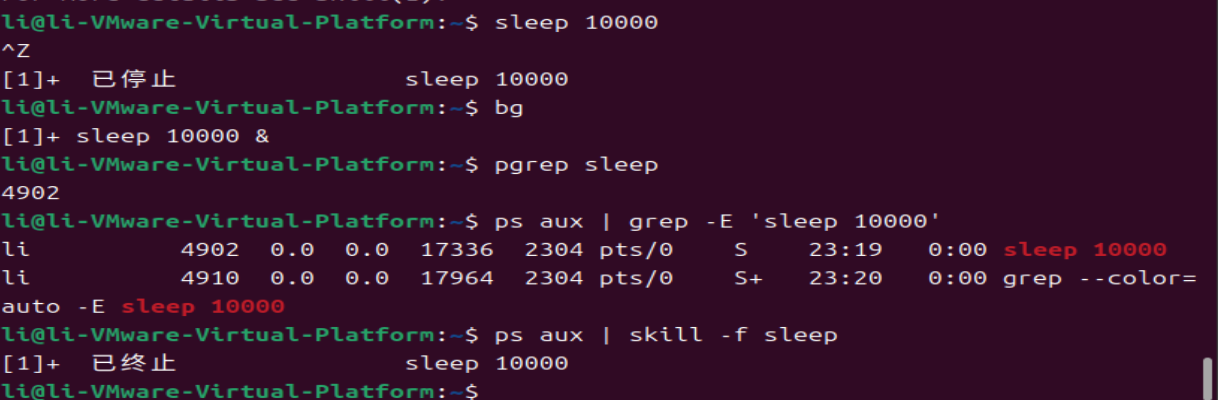
\includegraphics[width=1\textwidth]{屏幕截图 2024-09-12 232133.png}
  \caption{题目一}
    \end{figure}
\\
\\
\noindent 2.如果您希望某个进程结束后再开始另外一个进程, 应该如何实现呢?在这个练习中,我们使用 sleep 60 & 作为先执行的程序。一种方法是使用 wait 命令。尝试启动这个休眠命令,然后待其结束后再执行 ls 命令。

\begin{figure}[H]
  \centering
  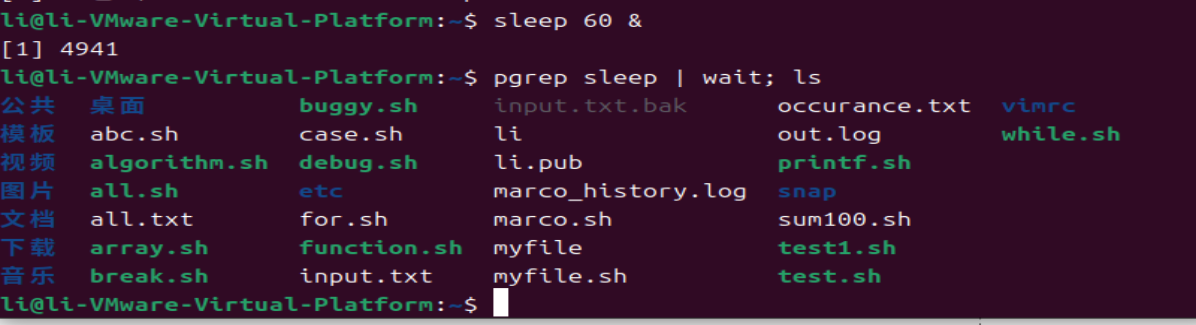
\includegraphics[width=1\textwidth]{屏幕截图 2024-09-12 232207.png}
  \caption{题目二}
    \end{figure}
\\
\\
\noindent 3.创建一个 dc 别名,它的功能是当我们错误的将 cd 输入为 dc 时也能正确执行。
\begin{figure}[H]
  \centering
  
\includegraphics[width=1\textwidth]{屏幕截图 2024-09-12 232321.png}
  \caption{题目三}
    \end{figure}
\\
\\
\noindent 4.执行 history | awk '{$1="";print substr($0,2)}' | sort | uniq -c | sort -n | tail -n 10 来获取您最常用的十条命令,尝试为它们创建别名。注意:这个命令只在 Bash 中生效,如果您使用 ZSH,使用 history 1 替换 history。
\begin{figure}[H]
  \centering
  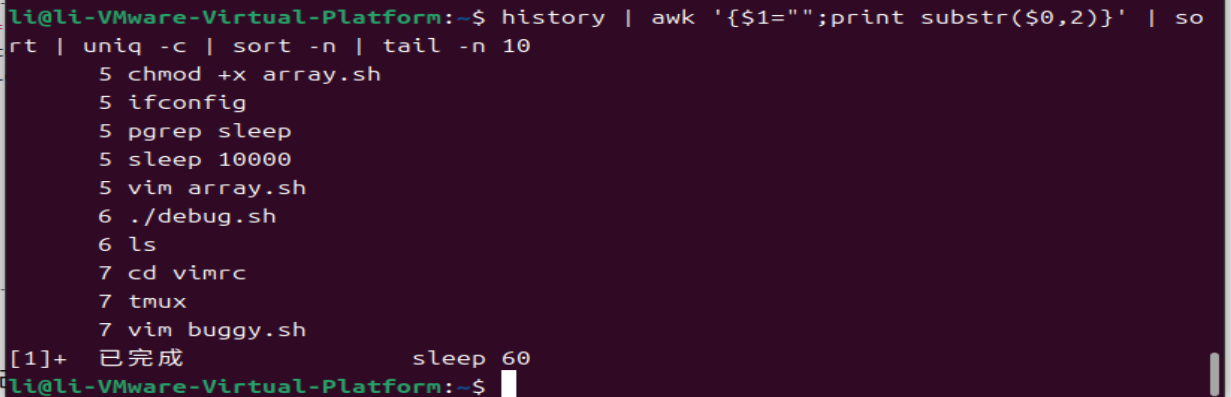
\includegraphics[width=1\textwidth]{屏幕截图 2024-09-12 232333.png}
  \caption{题目四}
    \end{figure}
\\
\\
% \vspace{-10pt}
\subsection{python入门基础练习}

\noindent 1.类的使用
 \begin{figure}[H]
  \centering
  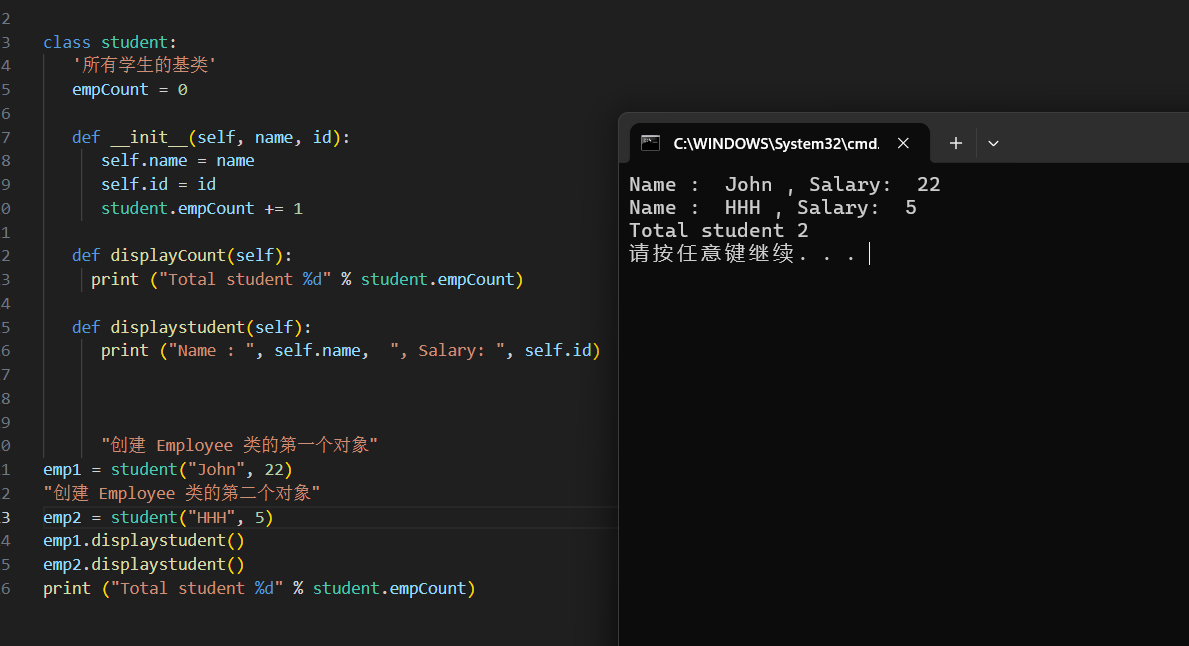
\includegraphics[width=1\textwidth]{屏幕截图 2024-09-12 120300.png}
  \caption{class}
    \end{figure}

\noindent 2.计算列表中每个偶数的平方并存储到一个新的列表。
\begin{figure}[H]
  \centering
  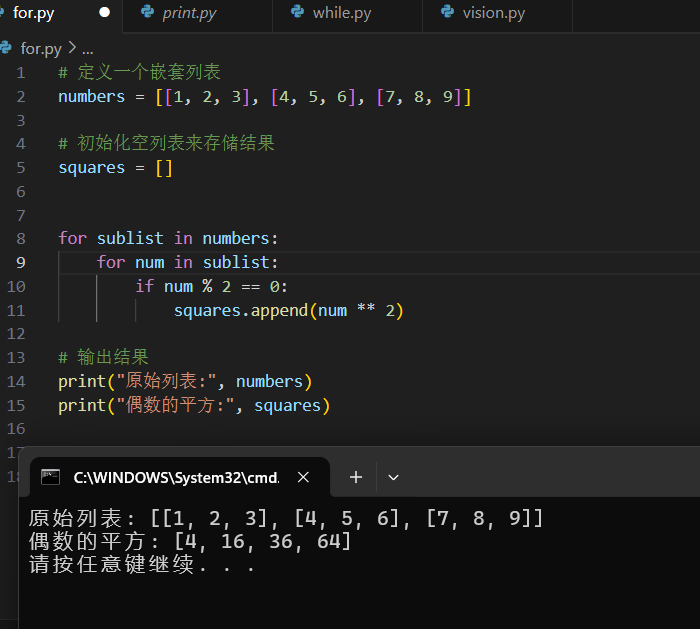
\includegraphics[width=1\textwidth]{屏幕截图 2024-09-06 105912.png}
  \caption{1}
    \end{figure}

3.输入1-100中的素数

\begin{figure}[H]
  \centering
  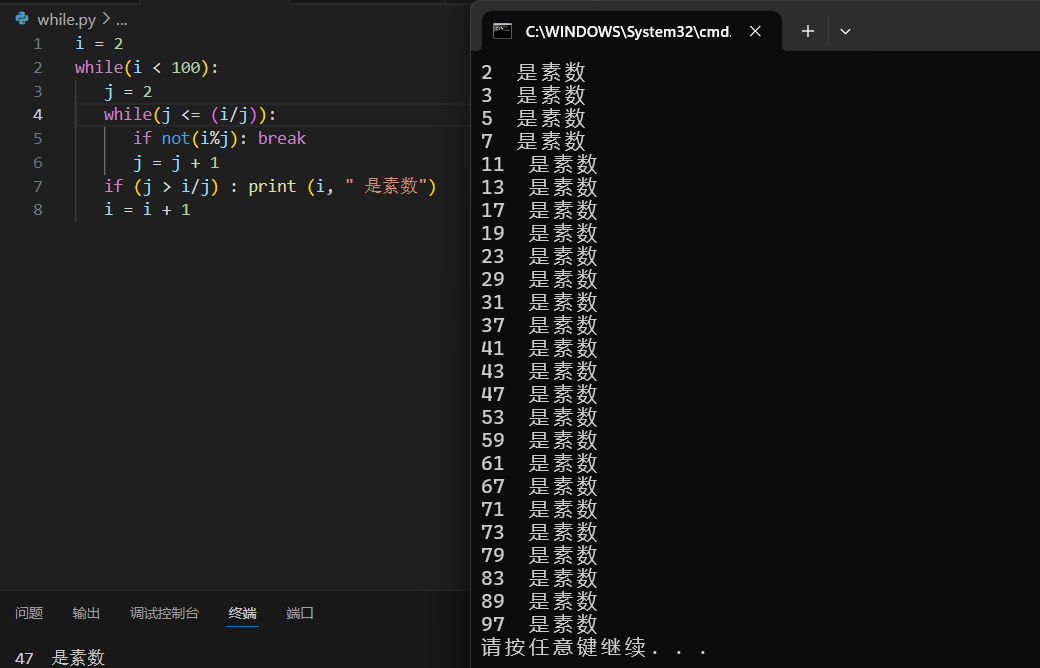
\includegraphics[width=1\textwidth]{屏幕截图 2024-09-06 145233.png}
  \caption{1}
    \end{figure}
\\
\subsection{python视觉应用练习}

\noindent 1.采用多种方法对图片进行颜色通道合并,如复制法、反射法、外包装法和常量法。
\begin{figure}[H]
  \centering
  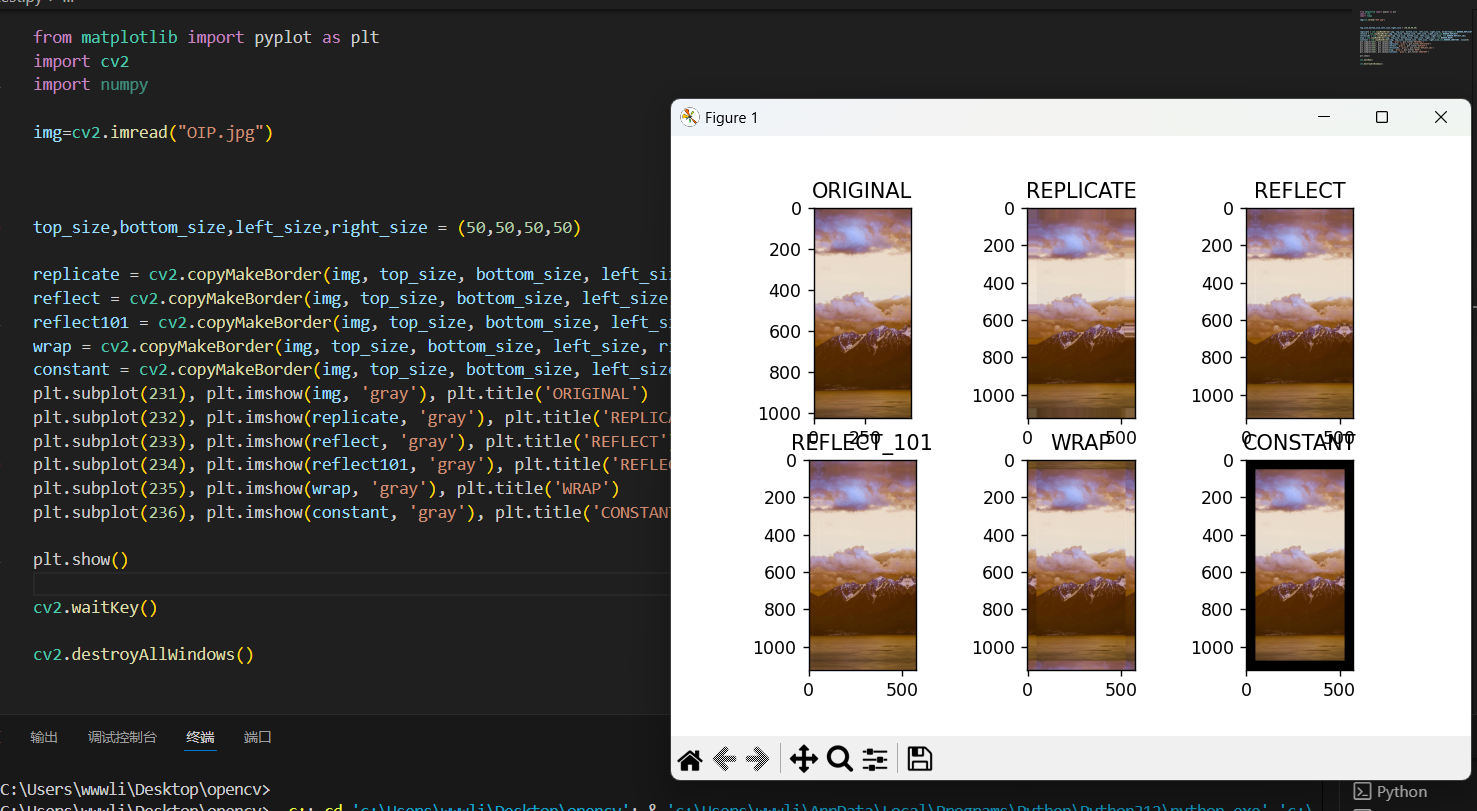
\includegraphics[width=1\textwidth]{屏幕截图 2024-09-12 171721.png}
  \caption{颜色通道合并}
    \end{figure}

2.将任意两张图片进行融合。
\begin{figure}[H]
  \centering
  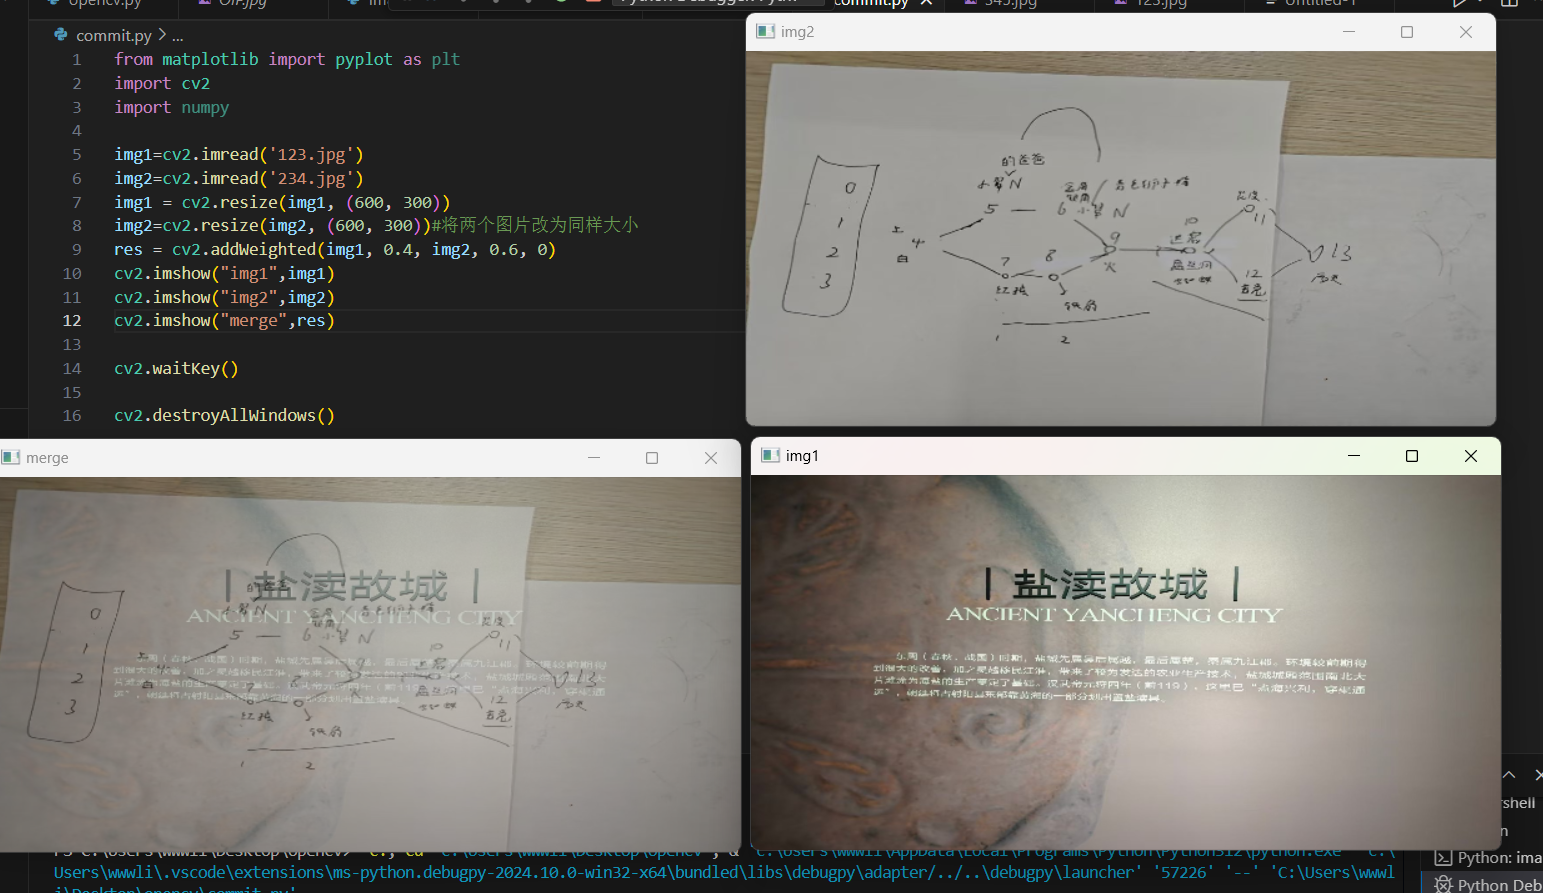
\includegraphics[width=1\textwidth]{屏幕截图 2024-09-12 191350.png}
  \caption{图片融合}
    \end{figure}


3.将图片进行腐蚀操作
\begin{figure}[H]
  \centering
  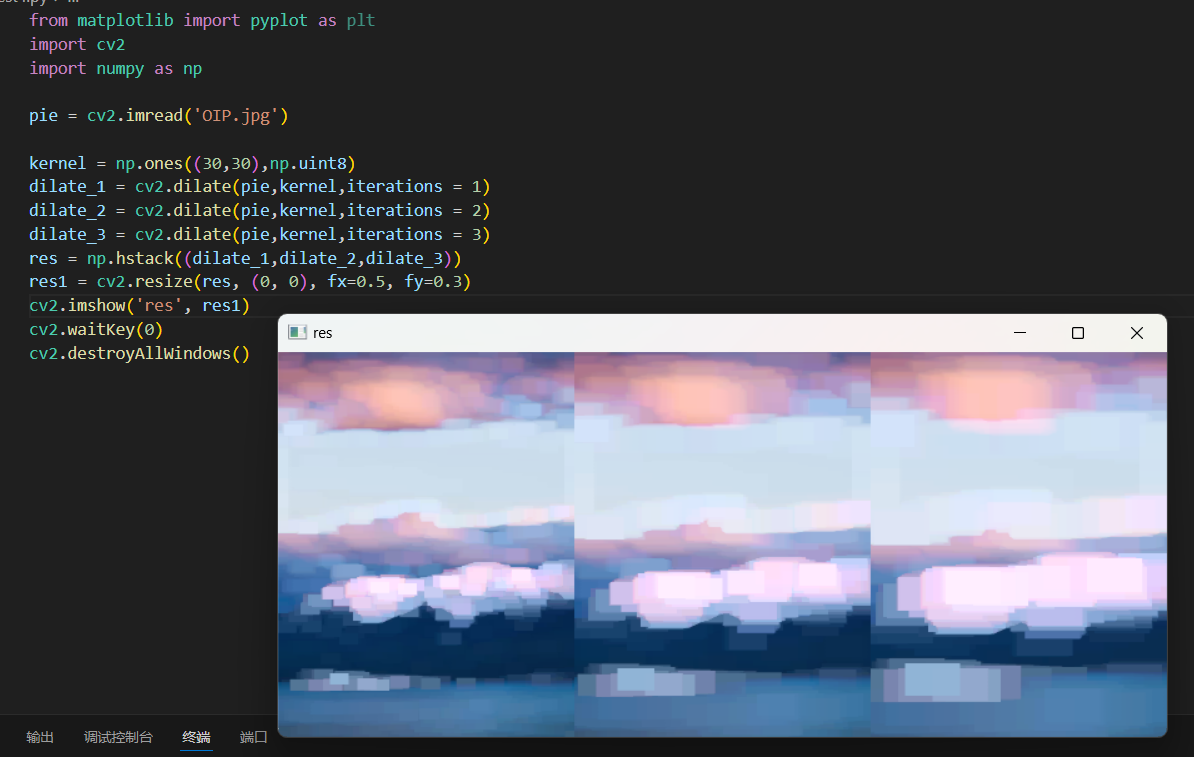
\includegraphics[width=\textwidth]{屏幕截图 2024-09-12 201525.png}
  \caption{图片的腐蚀操作}
\end{figure}

4.将图片进行膨胀操作
\begin{figure}[H]
  \centering
  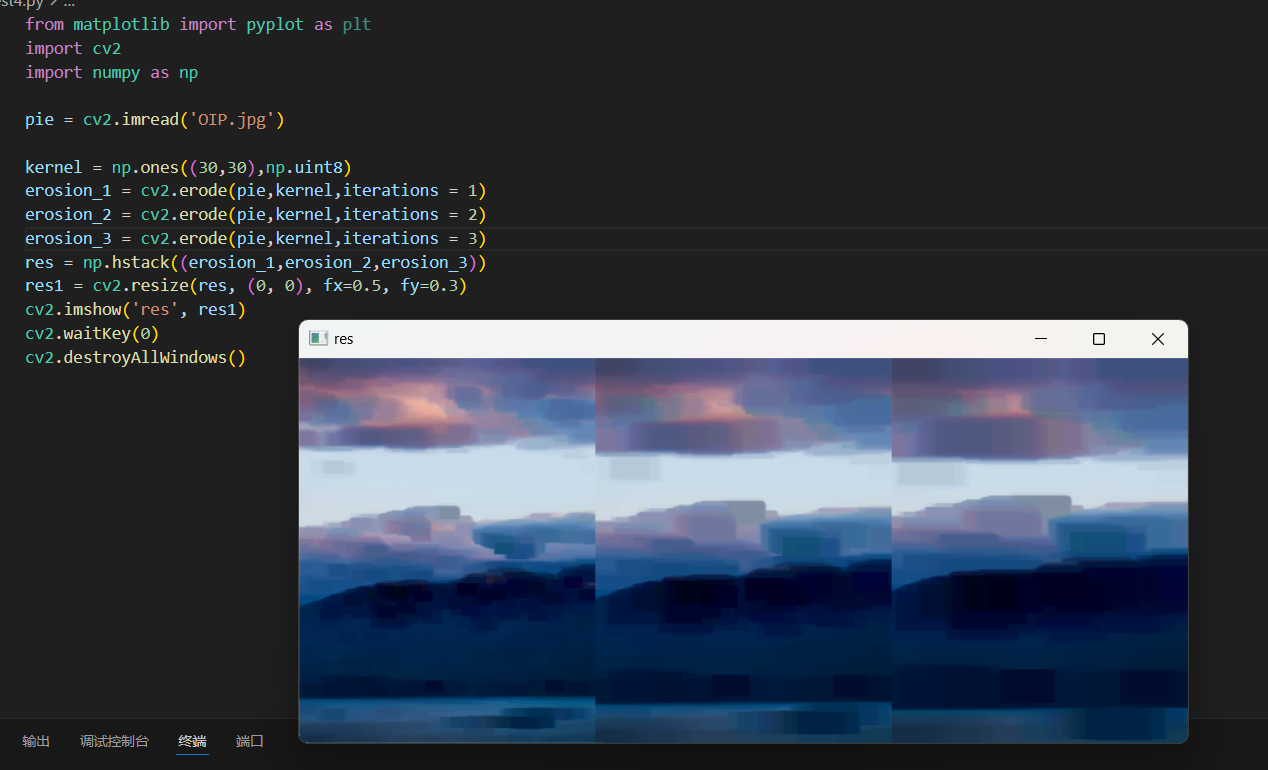
\includegraphics[width=\textwidth]{屏幕截图 2024-09-12 201917.png}
  \caption{膨胀}
\end{figure}


\section{实例展示}

\subsection{\color{green}命令行实例}
\begin{table}[H]
\centering
\caption{\color{red}命令行的实例展示大纲}
\begin{tabular}{ccc} 
\toprule

%\hline
 1&    tmux <C-b> \%         &  垂直分割                      \\ 
\hline
 2&<C-b> "   & 水平分割  \\ 
\hline
 3&<C-b> d  &   关闭tmux会话\\ 
\hline
 4& alias & 取别名  \\ 
\hline
 5&ifconfig & 显示网络设备  \\ 
\hline
 6& ssh +uesr + address&  配置ssh\\
 \hline

 7& pkill  -af sleep &   使用 pkill 结束进程\\
 \hline
8 &pgrep sleep 10000 &   查找 pid \\
 \hline
9 &pgrep sleep | wait; ls &   进程结束后再开始另外一个进程\\
 \hline
 10 & history | awk '{$1="";print substr($0,2)}' | sort | tail -n 10 &   获取最常用的十条命令\\
 %\hline
\bottomrule
\end{tabular}
\end{table}


1.使用tmux打开一个新的会话
\begin{figure}[H]
  \centering
  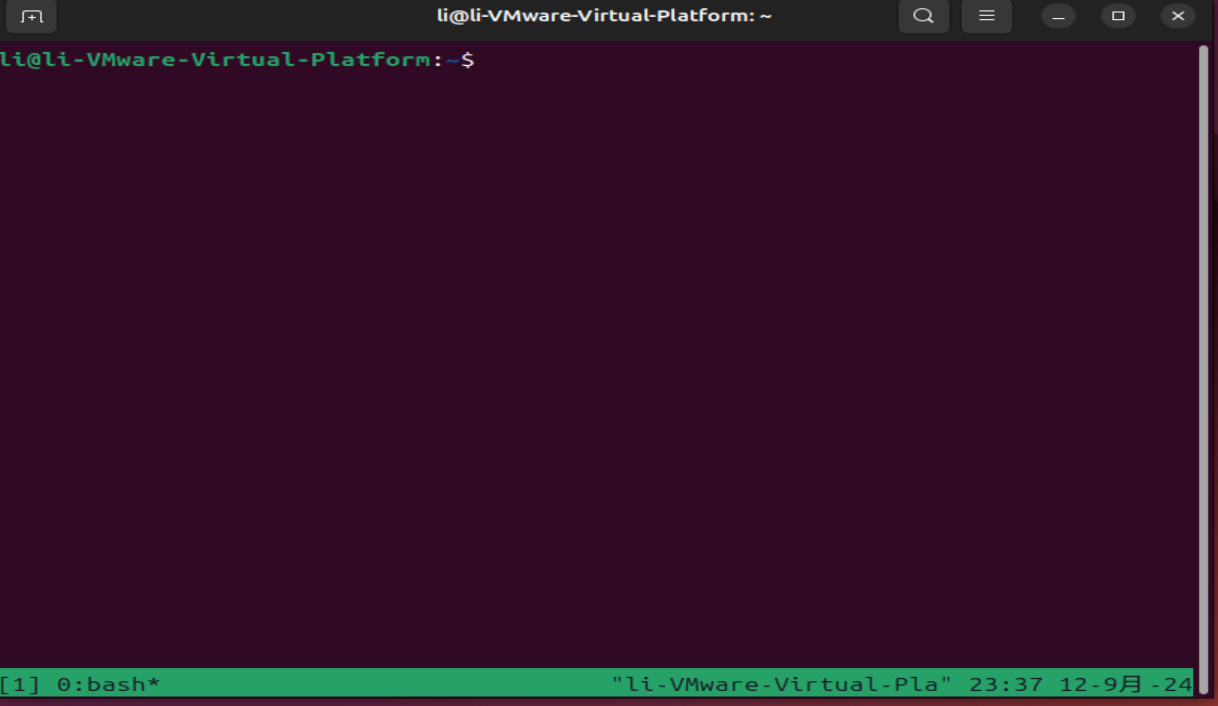
\includegraphics[width=\textwidth]{屏幕截图 2024-09-12 233752.png}
  \caption{tmux打开会话}
\end{figure}

2.tmux <C-b> \% 垂直分割
\begin{figure}[H]
  \centering
  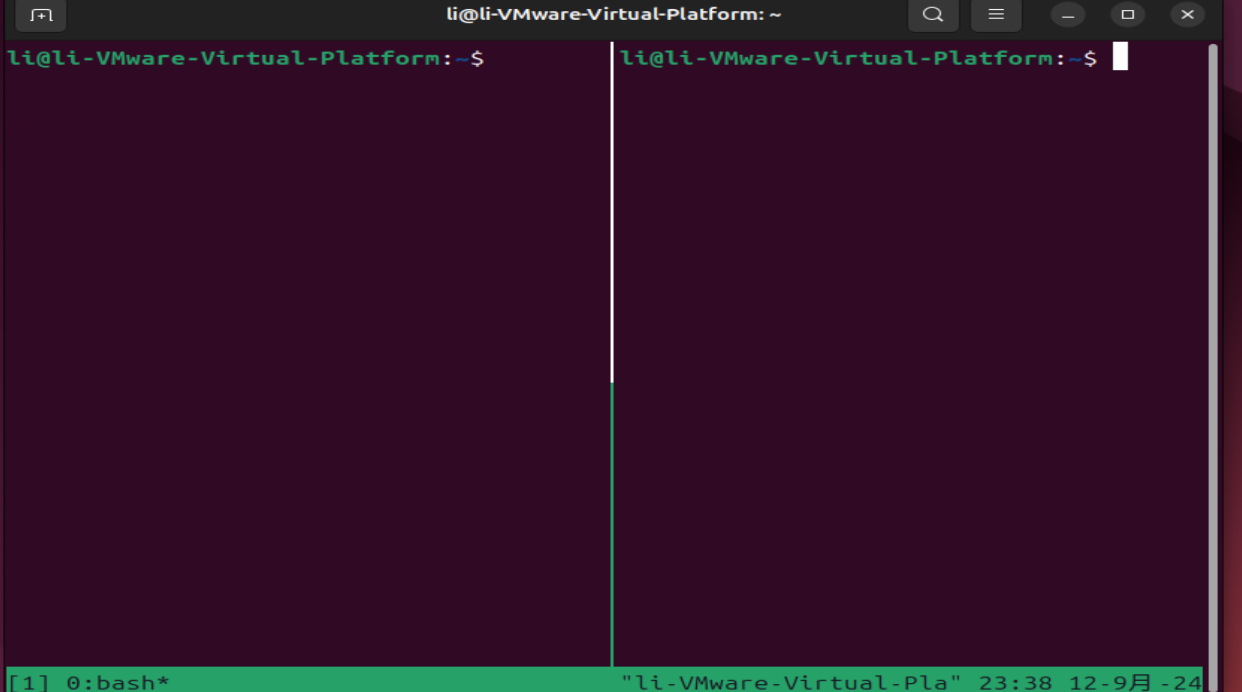
\includegraphics[width=\textwidth]{屏幕截图 2024-09-12 233822.png}
  \caption{tmux垂直分割}
\end{figure}


3.tmux <C-b> " 水平分割
\begin{figure}[H]
  \centering
  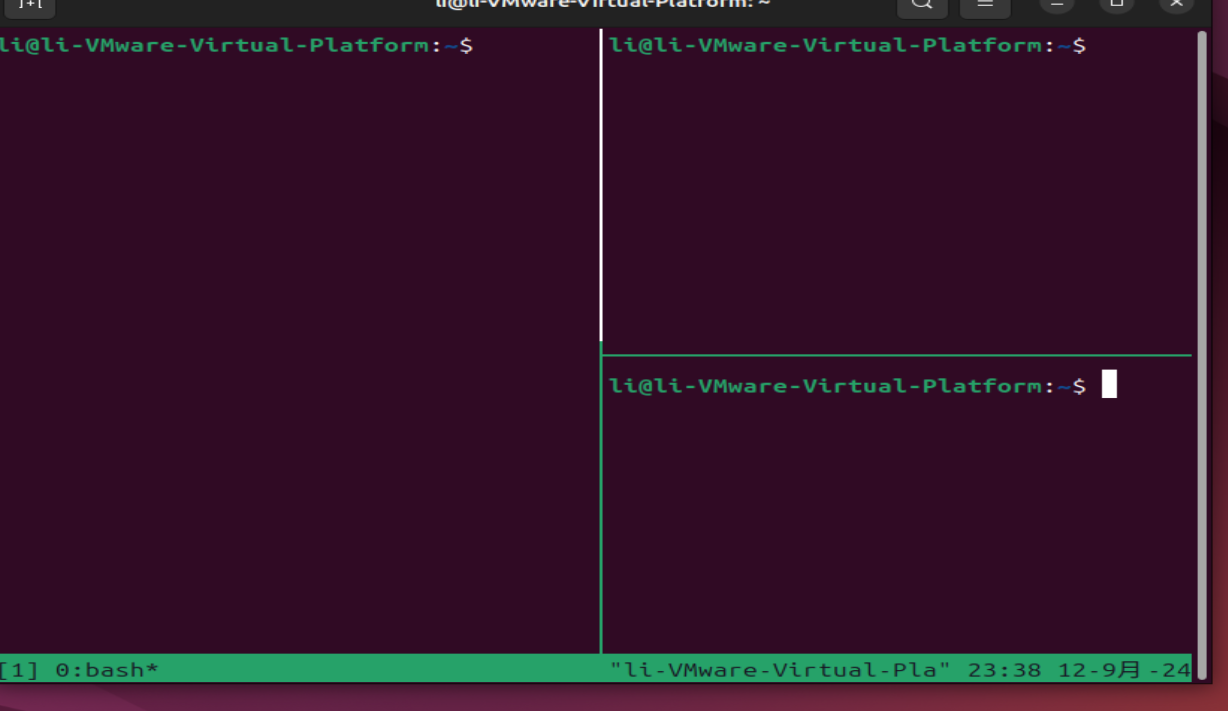
\includegraphics[width=\textwidth]{屏幕截图 2024-09-12 233838.png}
  \caption{tmux水平分割}
\end{figure}

4.tmux <C-b> d 关闭tmux会话
\begin{figure}[H]
  \centering
  
\includegraphics[width=\textwidth]{屏幕截图 2024-09-12 233853.png}
  \caption{关闭tmux会话}
\end{figure}




5.下载net-tools和openssh-server
\begin{figure}[H]
  \centering
  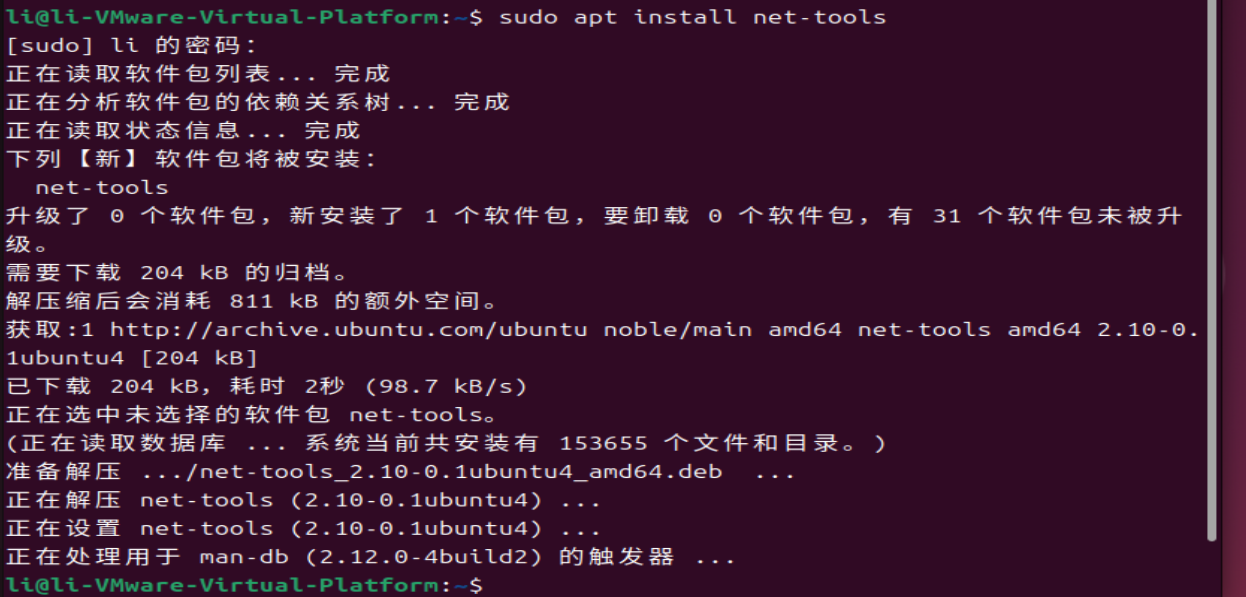
\includegraphics[width=\textwidth]{屏幕截图 2024-09-12 213056.png}
  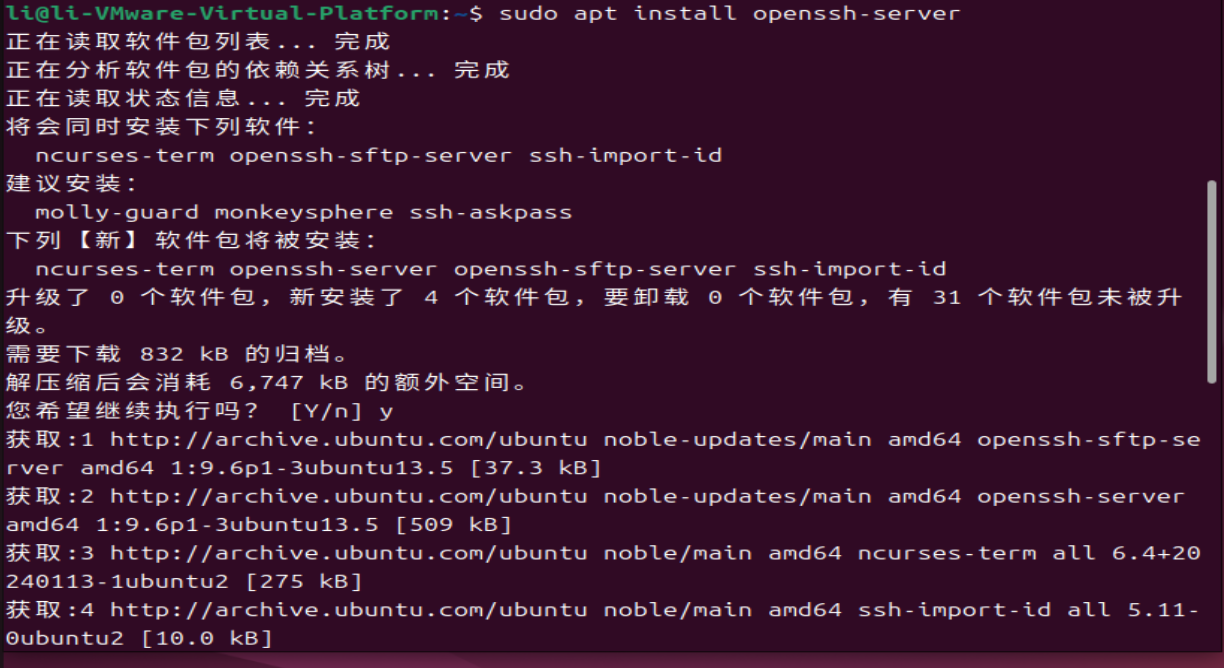
\includegraphics[width=\textwidth]{屏幕截图 2024-09-12 213734.png}
  \caption{下载ssh相关工具}
\end{figure}

6.ifconfig显示网络设备
\begin{figure}[H]
  \centering
  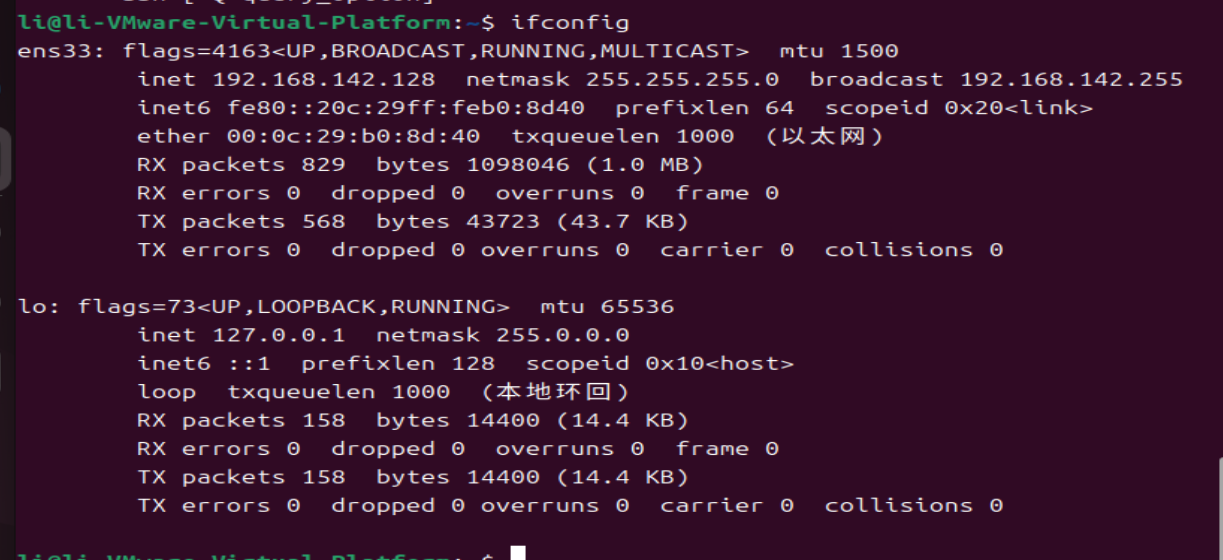
\includegraphics[width=\textwidth]{屏幕截图 2024-09-12 214319.png}
  \caption{ifconfig}
\end{figure}

7.配置ssh
\begin{figure}[H]
  \centering
  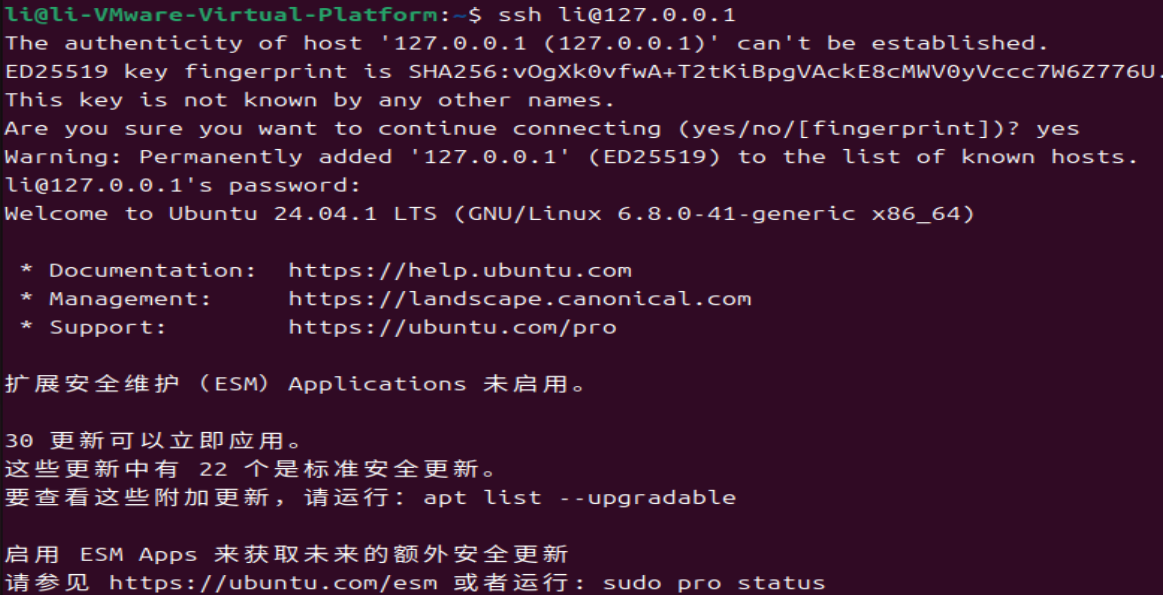
\includegraphics[width=\textwidth]{屏幕截图 2024-09-12 214404.png}
  \caption{配置ssh}
\end{figure}


\subsection{python基础实例展示}

\begin{table}[H]
\centering
\caption{\color{red}python基础的实例展示大纲}
\begin{tabular}{ccc} 
\toprule

%\hline
 1&   input/print        &  输入输出                     \\ 
\hline
 2&if-elif-else   & 条件语句  \\ 
\hline
 3& while/for &  循环语句\\ 
\hline
 4& for-for & 嵌套循环  \\ 
\hline
 5&class & 类的使用  \\ 
\hline
 6& break&  跳出循环\\
 \hline

 7& continue &  跳到循环起始点\\
 \hline
8 &function &   函数运用 \\
 \hline
9 &array &   数组的使用\\
 \hline
 10 & tup= (12,2,3,56) &   元组的使用\\
 11 & time.asctime() &  输出当前时间\\
 12 & tinydict={1: 'a',2:'b'} &   字典的使用\\
 13 & import re &   正则表达式\\

 %\hline
\bottomrule
\end{tabular}
\end{table}

1.输入输出
\begin{figure}[H]
  \centering
  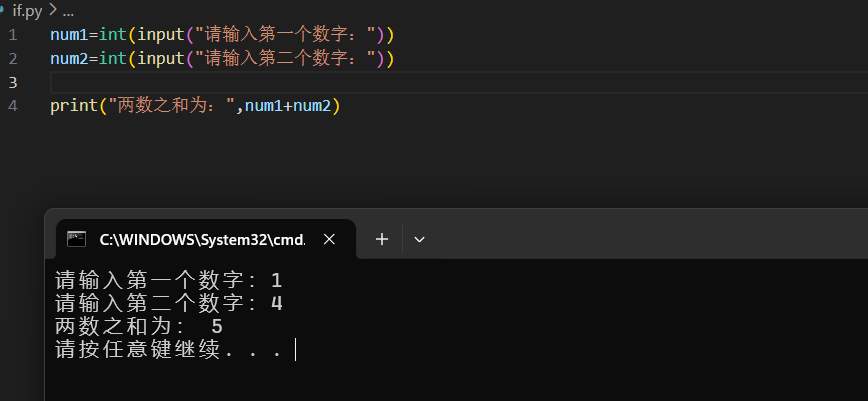
\includegraphics[width=1\textwidth]{屏幕截图 2024-09-11 214843.png}
  \caption{输入输出}
    \end{figure}

2.if-elif-else
\begin{figure}[H]
  \centering
  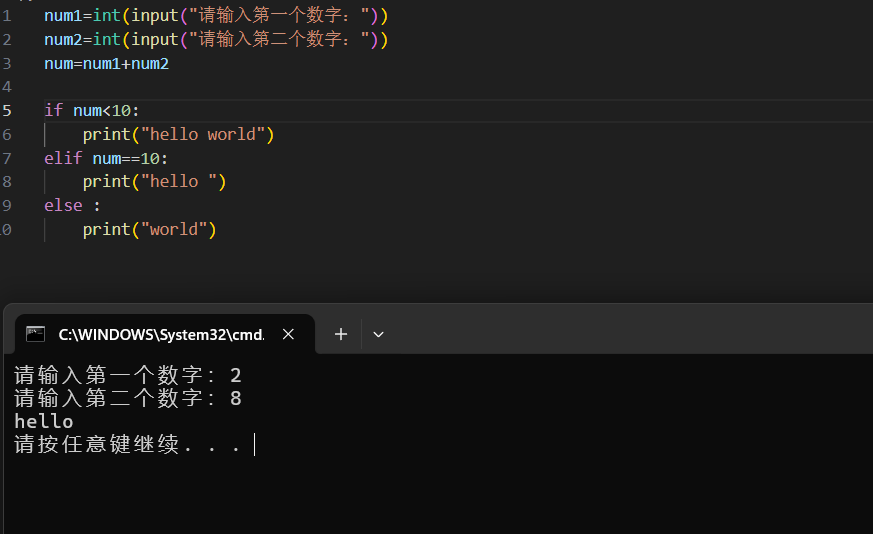
\includegraphics[width=1\textwidth]{屏幕截图 2024-09-11 215453.png}
  \caption{条件语句}
    \end{figure}

3.循环语句
\begin{figure}[H]
  \centering
  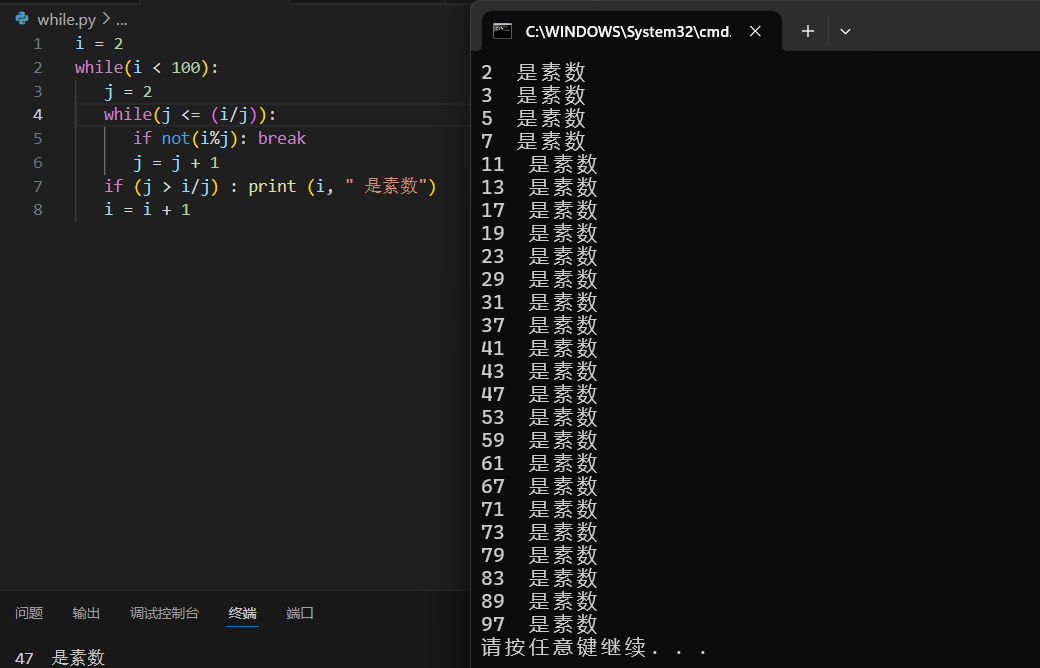
\includegraphics[width=1\textwidth]{屏幕截图 2024-09-06 145233.png}
  \caption{循环语句}
    \end{figure}


4.嵌套循环
    \begin{figure}[H]
  \centering
  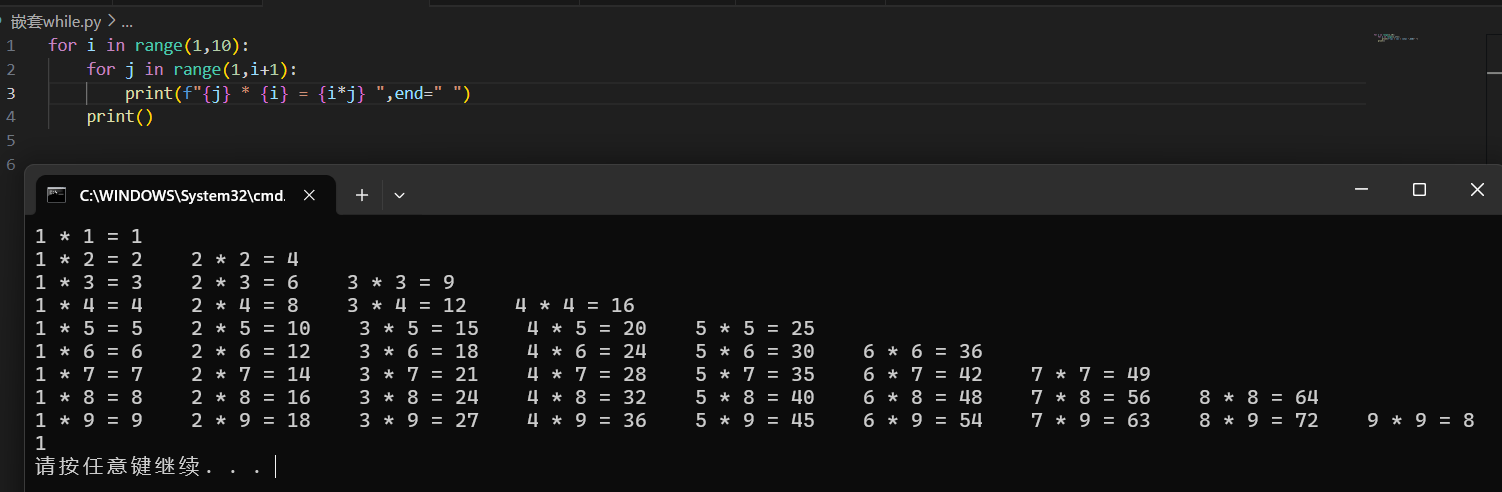
\includegraphics[width=1\textwidth]{屏幕截图 2024-09-12 101626.png}
  \caption{嵌套循环}
    \end{figure}

5.类的使用
 \begin{figure}[H]
  \centering
  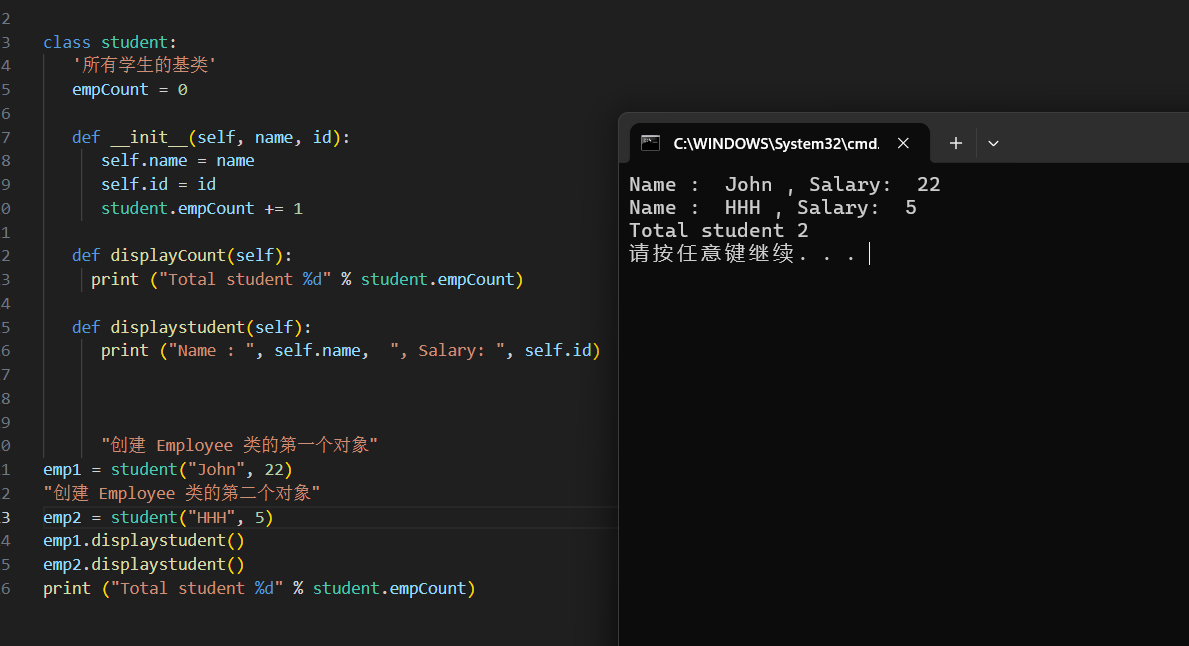
\includegraphics[width=1\textwidth]{屏幕截图 2024-09-12 120300.png}
  \caption{class}
    \end{figure}

6.break跳出循环
 \begin{figure}[H]
  \centering
  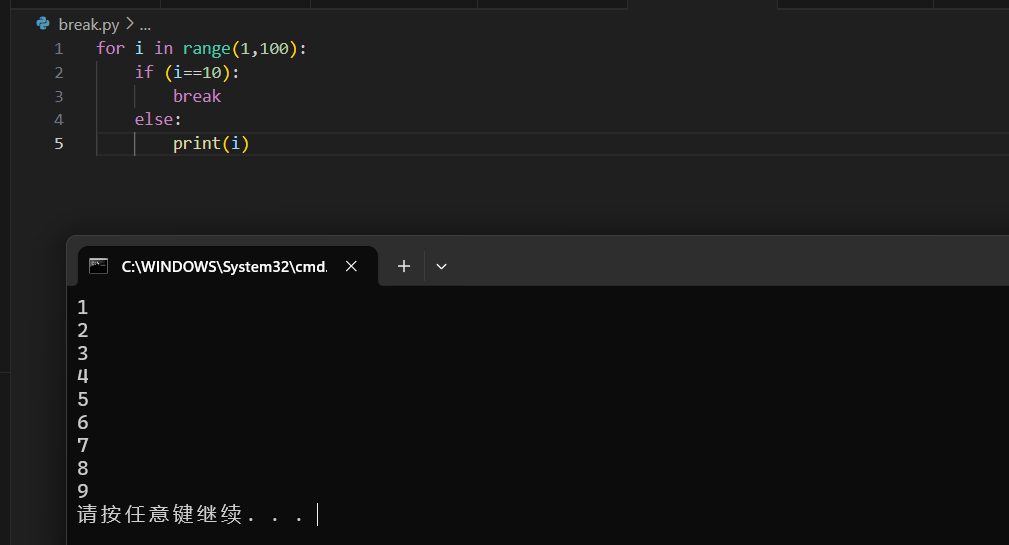
\includegraphics[width=1\textwidth]{屏幕截图 2024-09-12 102808.png}
  \caption{break}
    \end{figure}

7.continue输出奇数
 \begin{figure}[H]
  \centering
  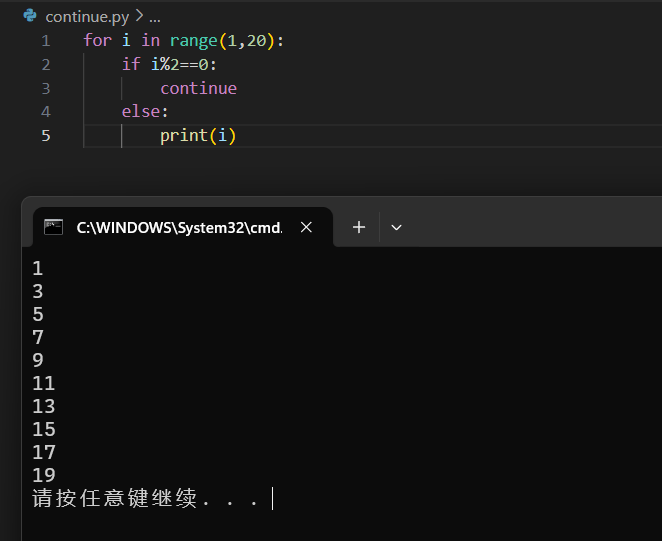
\includegraphics[width=1\textwidth]{屏幕截图 2024-09-12 104528.png}
  \caption{continue}
    \end{figure}

8.函数运用
 \begin{figure}[H]
  \centering
  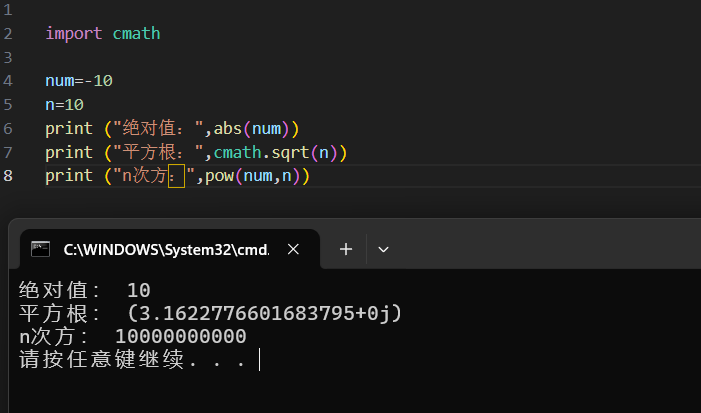
\includegraphics[width=1\textwidth]{屏幕截图 2024-09-12 110705.png}
  \caption{数学函数运用}
    \end{figure}

9.数组的基本用法
 \begin{figure}[H]
  \centering
  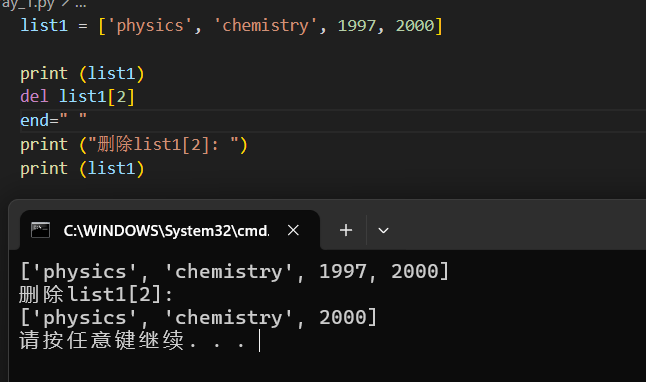
\includegraphics[width=1\textwidth]{屏幕截图 2024-09-12 112311.png}
  \caption{数组}
    \end{figure}

10.元组的基本语句
 \begin{figure}[H]
  \centering
  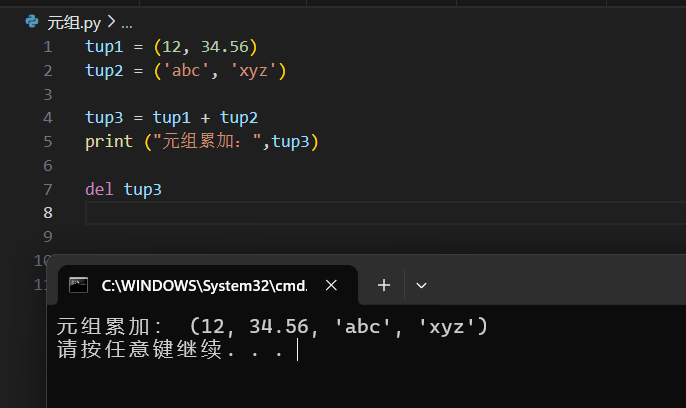
\includegraphics[width=1\textwidth]{屏幕截图 2024-09-12 113011.png}
  \caption{元组}
    \end{figure}

    
11.time的基本语句
     \begin{figure}[H]
  \centering
  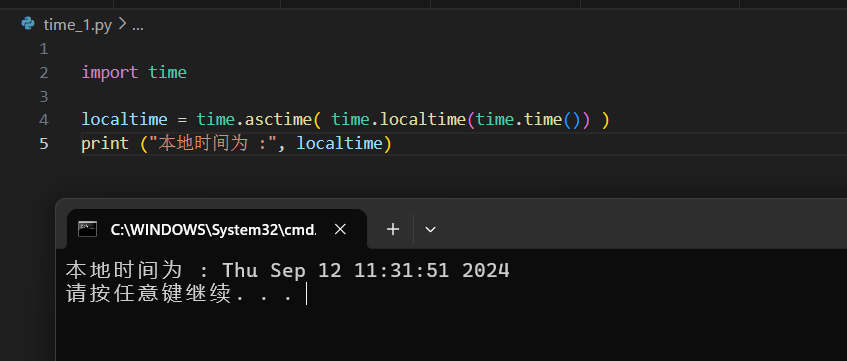
\includegraphics[width=1\textwidth]{屏幕截图 2024-09-12 113159.png}
  \caption{time的基本语句}
    \end{figure}

12.字典的基本语句
 \begin{figure}[H]
  \centering
  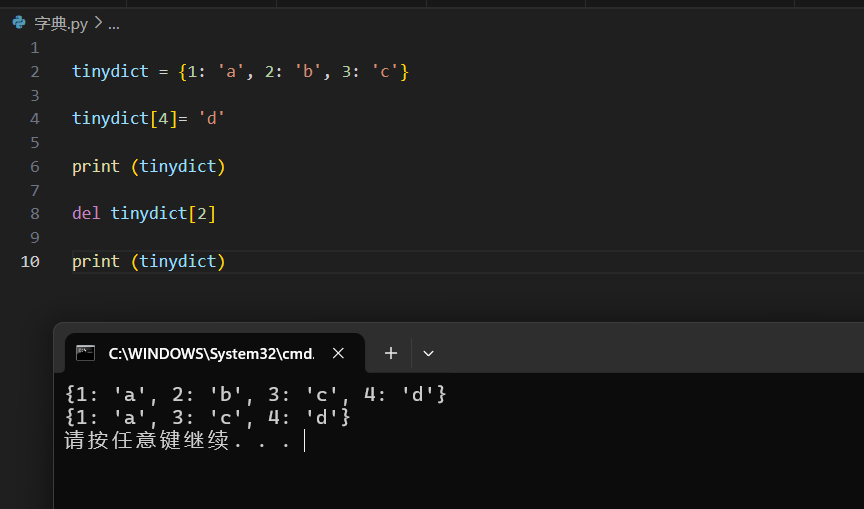
\includegraphics[width=1\textwidth]{屏幕截图 2024-09-12 113929.png}
  \caption{字典的基本语句}
    \end{figure}


13.正则表达式
 \begin{figure}[H]
  \centering
  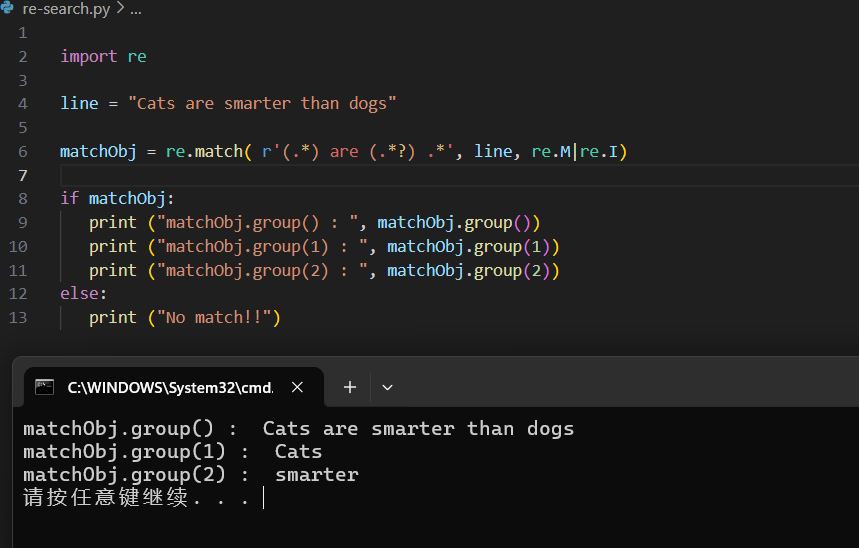
\includegraphics[width=1\textwidth]{屏幕截图 2024-09-12 135504.png}
  \caption{正则表达式}
    \end{figure}
    
\subsection{\color{green}python视觉应用实例展示}


\begin{table}[H]
\centering
\caption{python基础的实例展示大纲\color{red}(这里只显示部分代码,详细看图片内容)}
\begin{tabular}{ccc} 
\toprule

%\hline
 1&   cv2.imread()       &  读入图片                    \\ 
\hline
 2&cv2.imshow()   & 输出图片\\ 
\hline
 3&camera=cv2.VideoCapture("camera1.mp4") &  读入视频\\ 
\hline
 4& cv2.VideoWriter("abc.avi",cv2.VideoWriter_fourcc('I','4','2','0'),fps,size) & 转换视频格式  \\ 
\hline
 5&cv2.copyMakeBorder() & 颜色通道合并  \\ 
\hline
 6& ret, thresh2 = cv2.threshold(img, 127, 255, cv2.THRESH_BINARY_INV)&  图片阈值\\
 \hline

 7&cv2.addWeighted(img1, 0.4, img2, 0.6, 0)&  图片融合\\
 \hline
8 & cv2.resize(img, (0, 0), fx=0.5, fy=0.3) &   改变图片比例 \\
 \hline
9 &cv2.GaussianBlur(img, (5, 5), 1)  &   图片平滑\\
 \hline
 10 &np.hstack((dilate,erosion)) &   图片腐蚀\\
 11 & hsv=cv2.cvtColor(res,cv2.COLOR_BGR2HSV) &  图片转化为hsv\\
 12 & plt.subplot(231), plt.imshow(img, 'gray'), plt.title('ORIGINAL') &   图片展示\\
 13 & np.hstack((dilate,erosion)) &   图片的梯度操作\\

 %\hline
\bottomrule
\end{tabular}
\end{table}


1.读入图片
\begin{figure}[H]
  \centering
  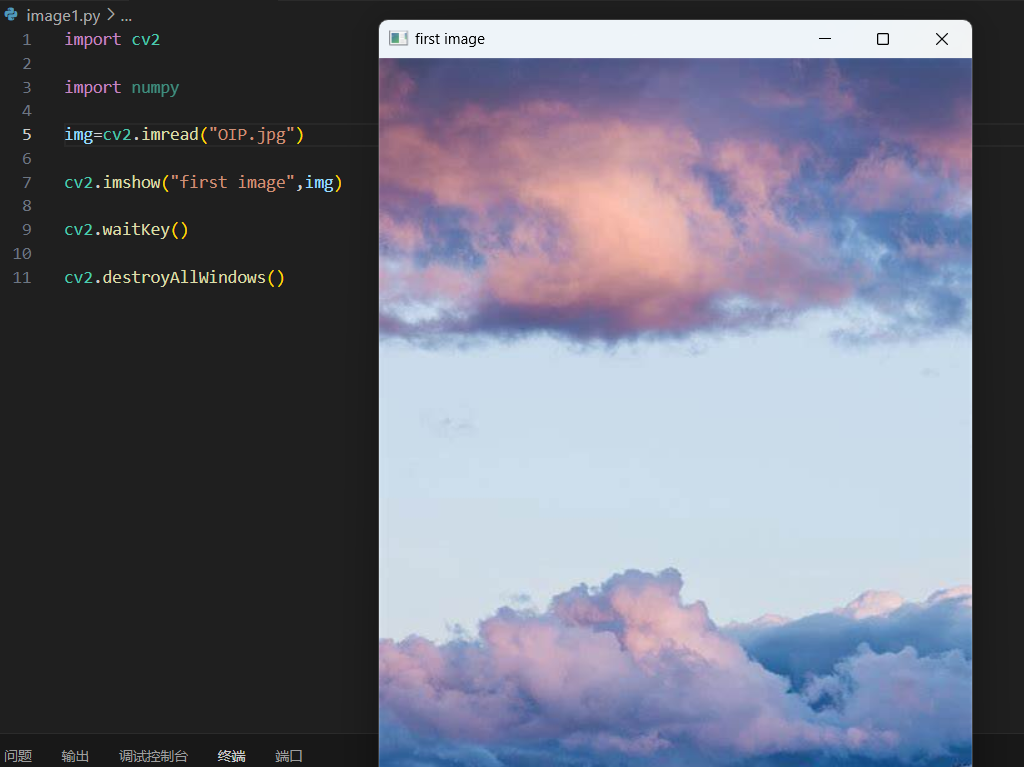
\includegraphics[width=1\textwidth]{屏幕截图 2024-09-12 151958.png}
  \caption{读入图片}
    \end{figure}

2.使图片成为灰色图像
\begin{figure}[H]
  \centering
  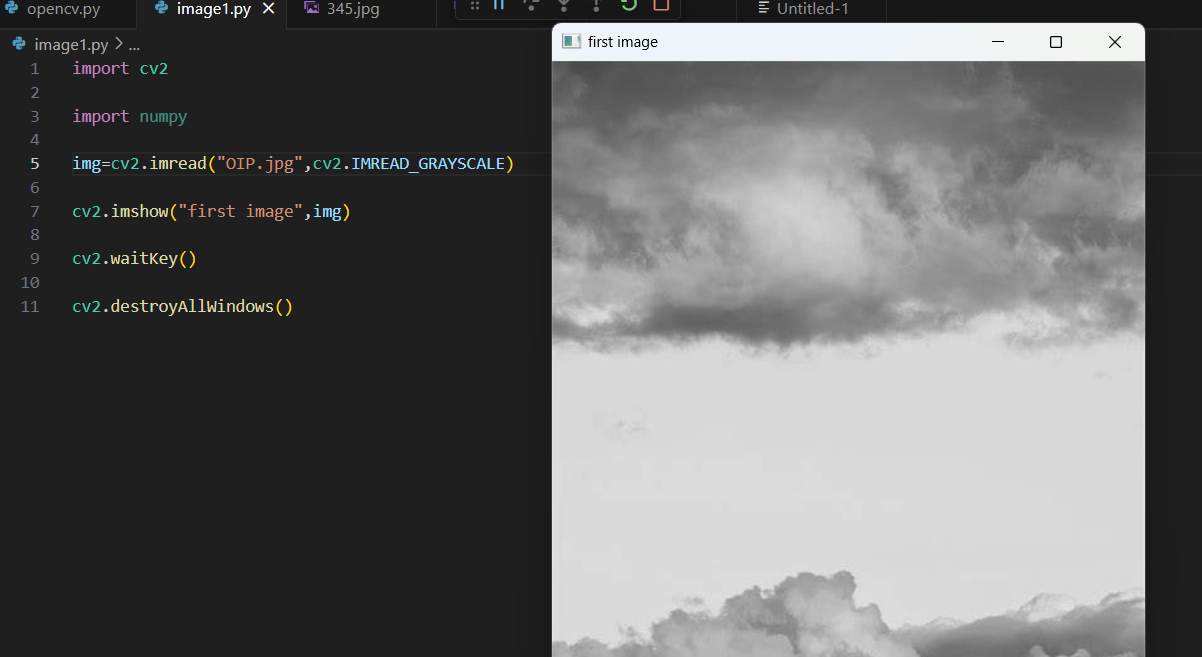
\includegraphics[width=1\textwidth]{屏幕截图 2024-09-12 153303.png}
  \caption{灰色图像}
    \end{figure}



3.读入视频并且播放
\begin{figure}[H]
  \centering
  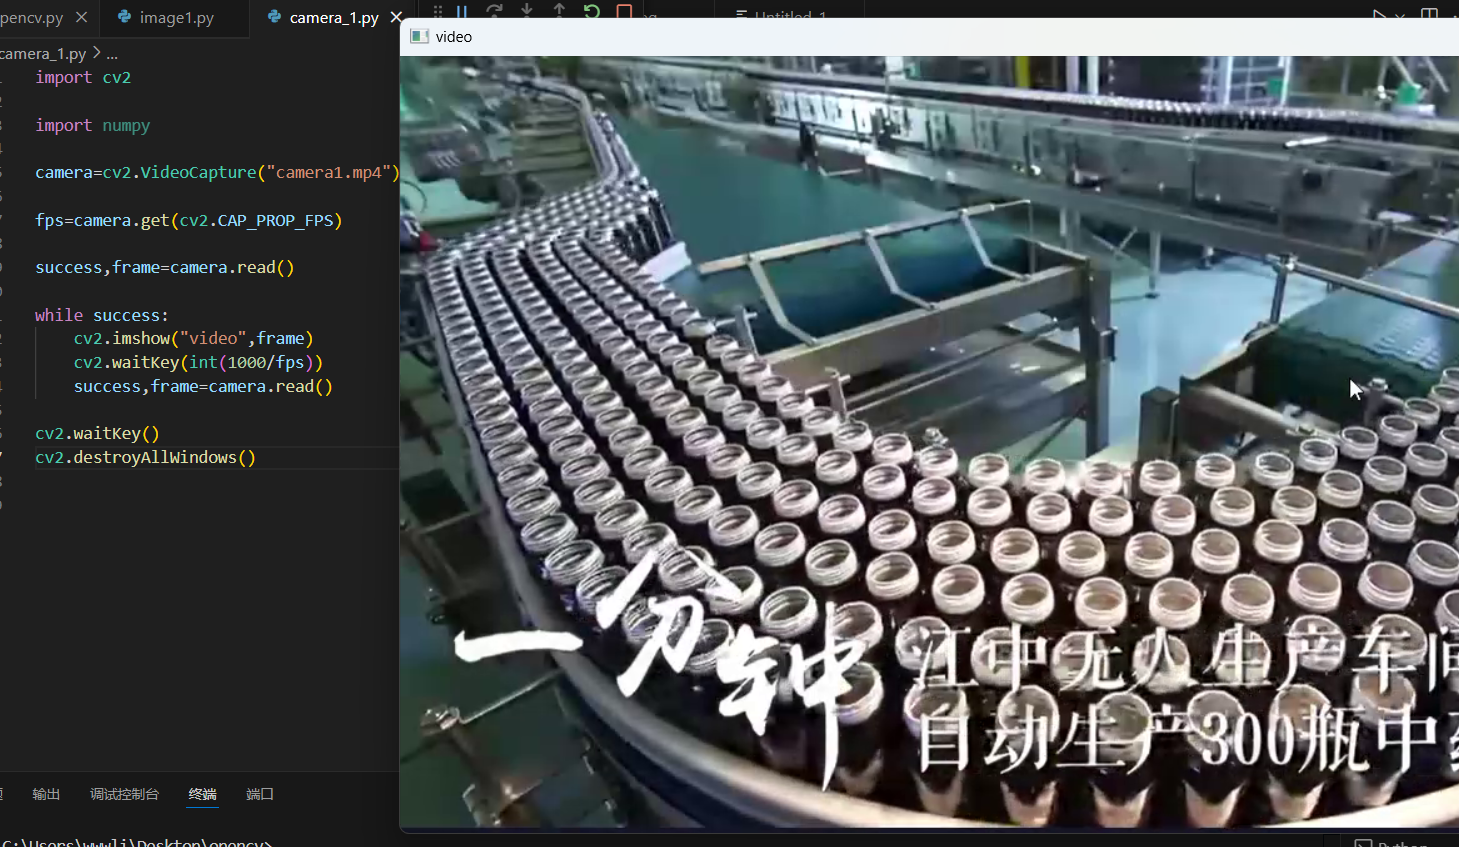
\includegraphics[width=1\textwidth]{屏幕截图 2024-09-12 154925.png}
  \caption{读入视频}
    \end{figure}

4.转换视频格式成.avi
\begin{figure}[H]
  \centering
  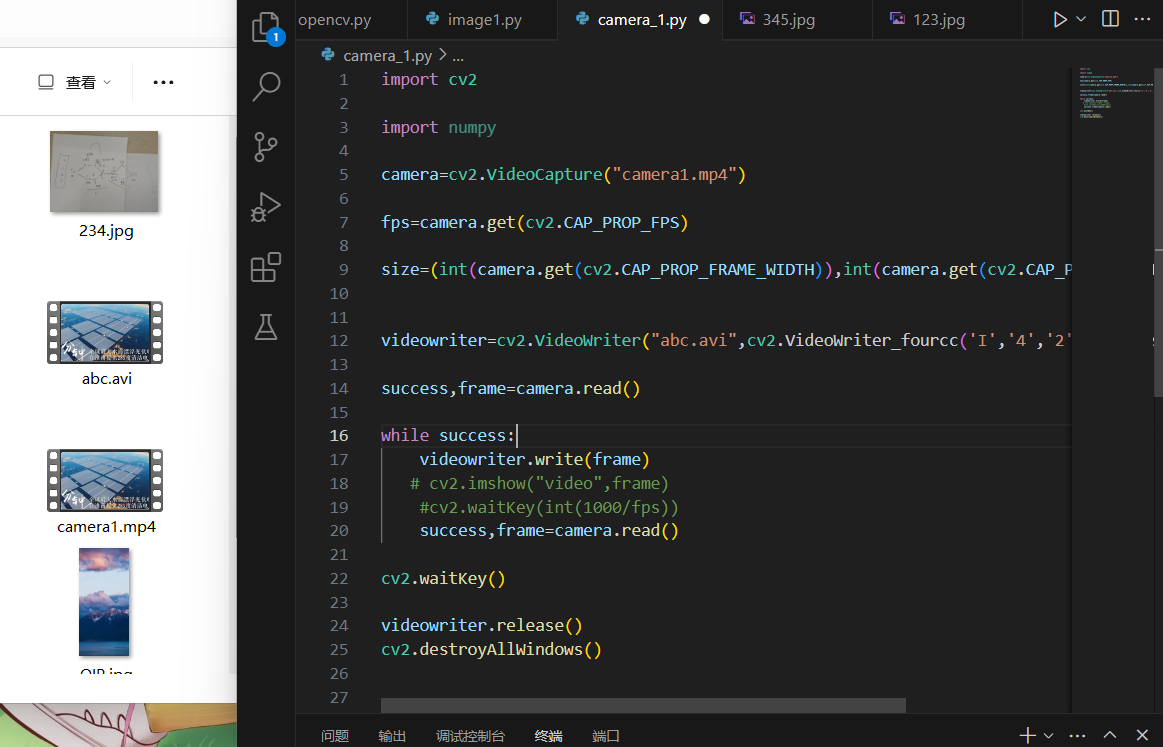
\includegraphics[width=1\textwidth]{屏幕截图 2024-09-12 160329.png}
  \caption{转换视频格式}
    \end{figure}

5.输入特定位置的图片
\begin{figure}[H]
  \centering
  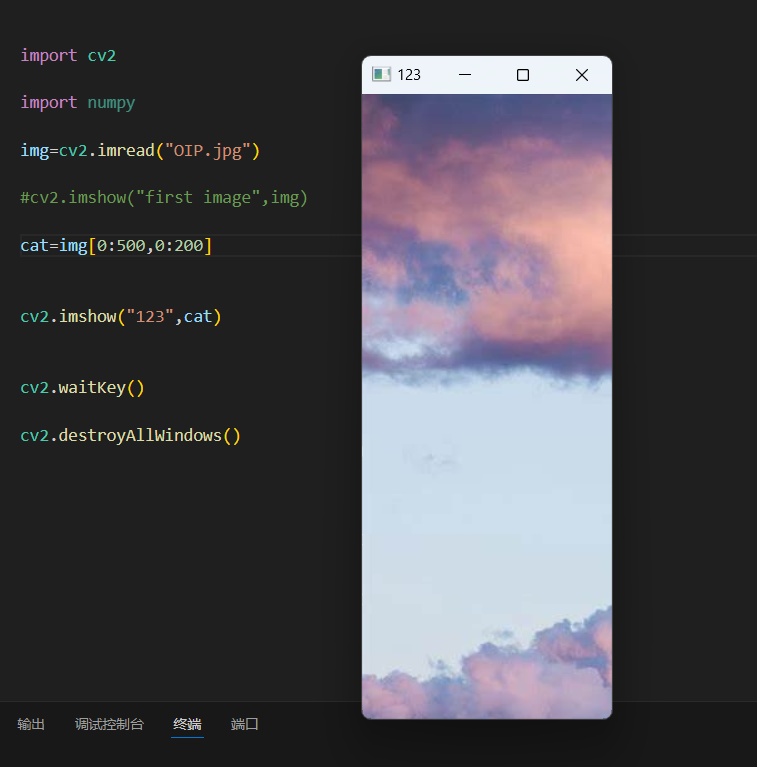
\includegraphics[width=1\textwidth]{屏幕截图 2024-09-12 164317.png}
  \caption{输入特定位置的图片}
    \end{figure}

6.采用多种方法对图片进行颜色通道合并,如复制法、反射法、外包装法和常量法。
\begin{figure}[H]
  \centering
  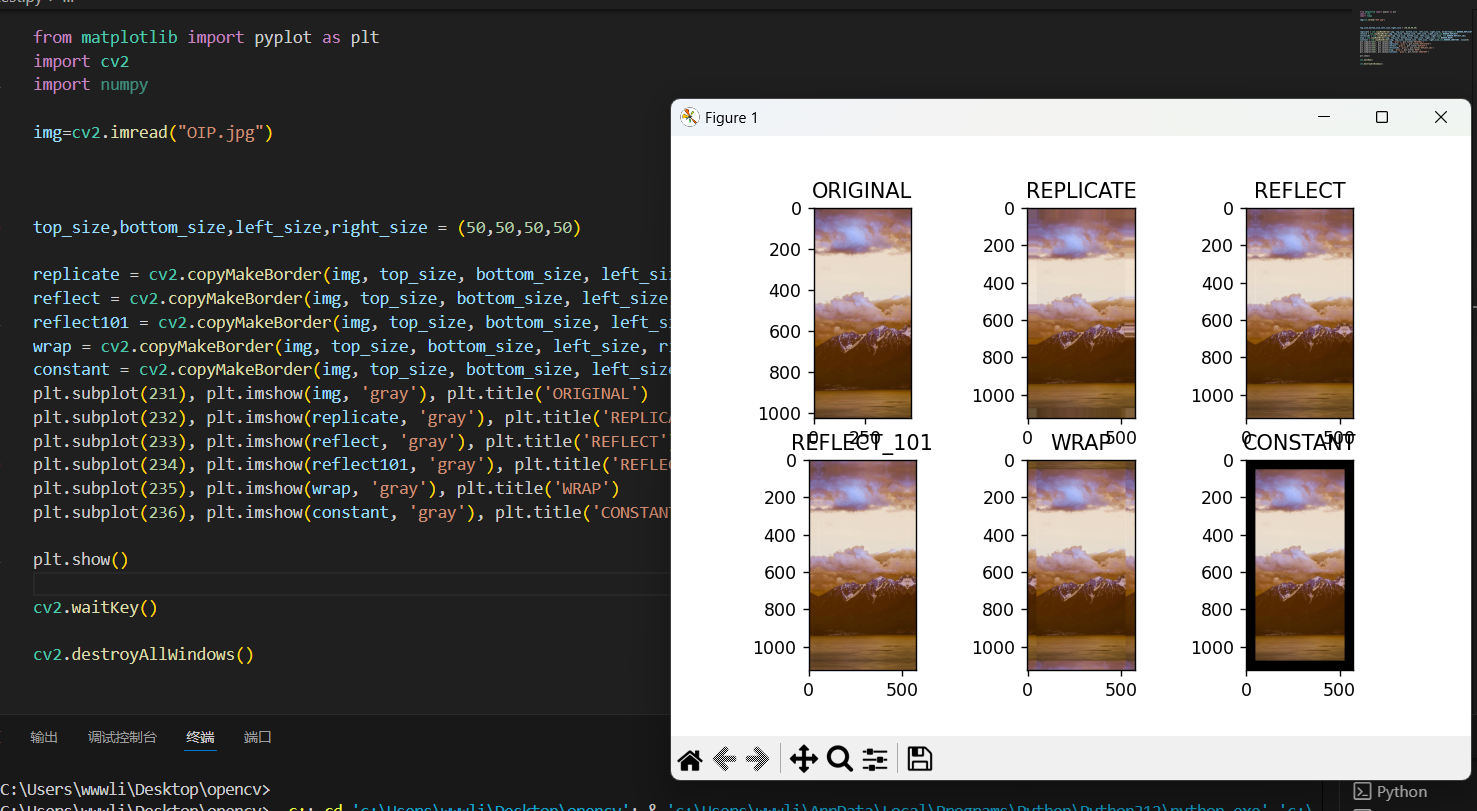
\includegraphics[width=1\textwidth]{屏幕截图 2024-09-12 171721.png}
  \caption{颜色通道合并}
    \end{figure}

7.图片融合
\begin{figure}[H]
  \centering
  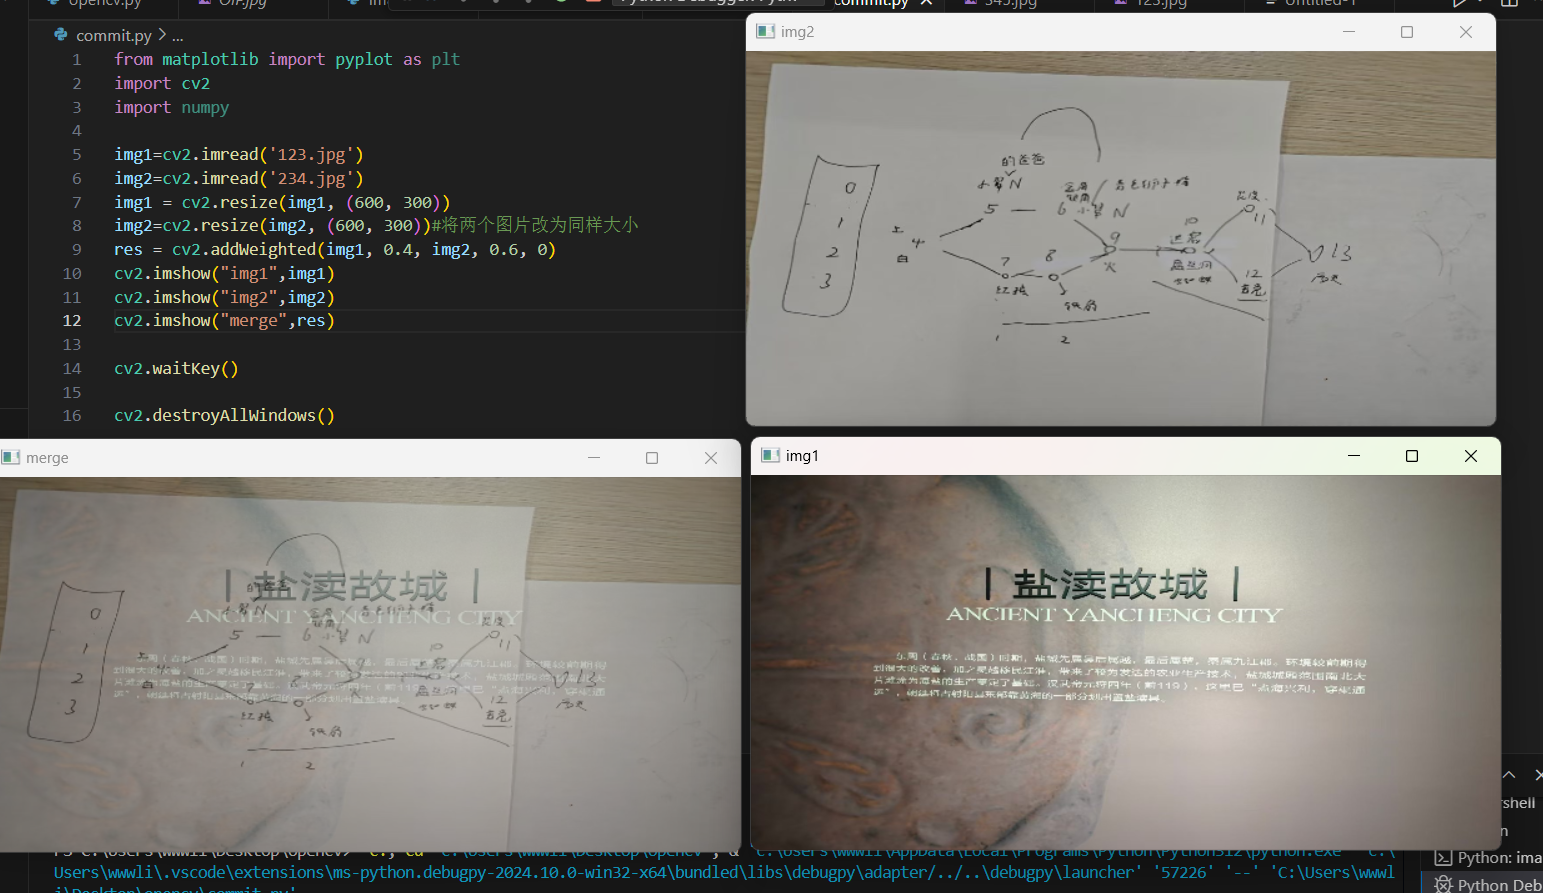
\includegraphics[width=1\textwidth]{屏幕截图 2024-09-12 191350.png}
  \caption{图片融合}
    \end{figure}



8.改变图片长宽比
\begin{figure}[H]
  \centering
  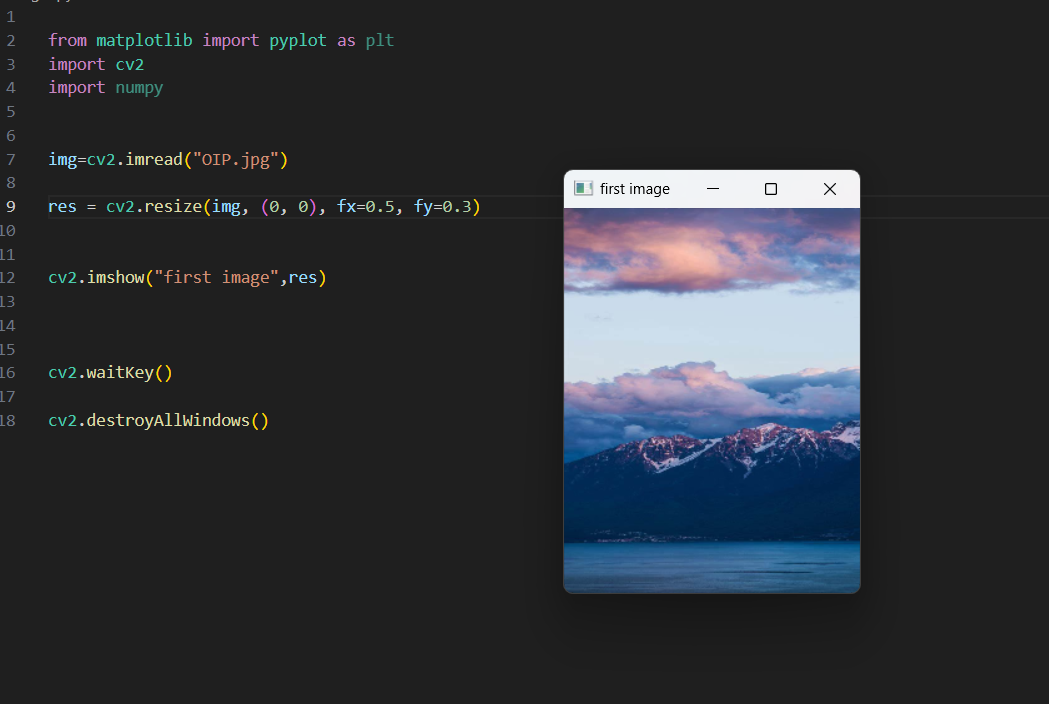
\includegraphics[width=1\textwidth]{屏幕截图 2024-09-12 192504.png}
  \caption{改变图片长宽比}
    \end{figure}

9.图片转为hsv
\begin{figure}[H]
  \centering
  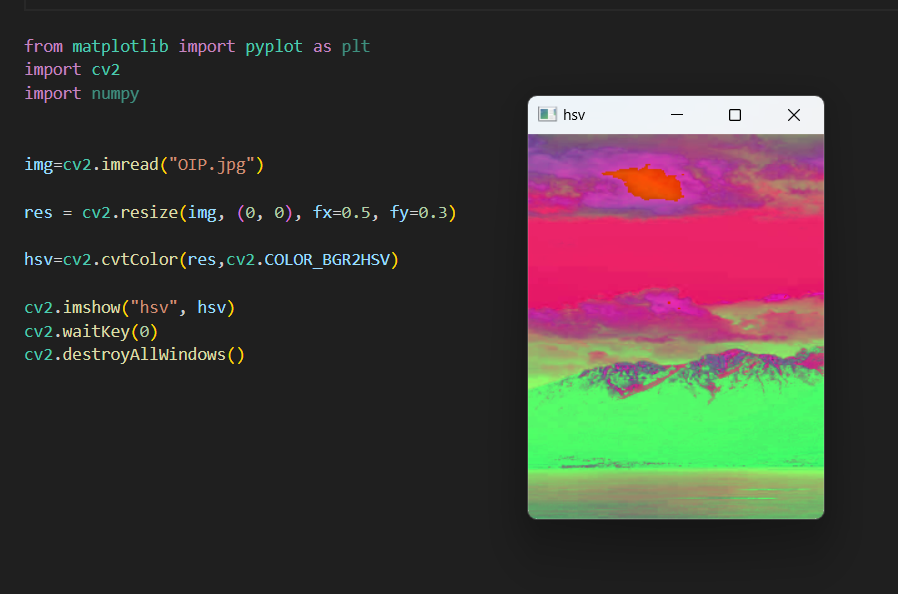
\includegraphics[width=1\textwidth]{屏幕截图 2024-09-12 192953.png}
  \caption{图片转为hsv}
    \end{figure}

10.图片阈值
\begin{figure}[H]
  \centering
  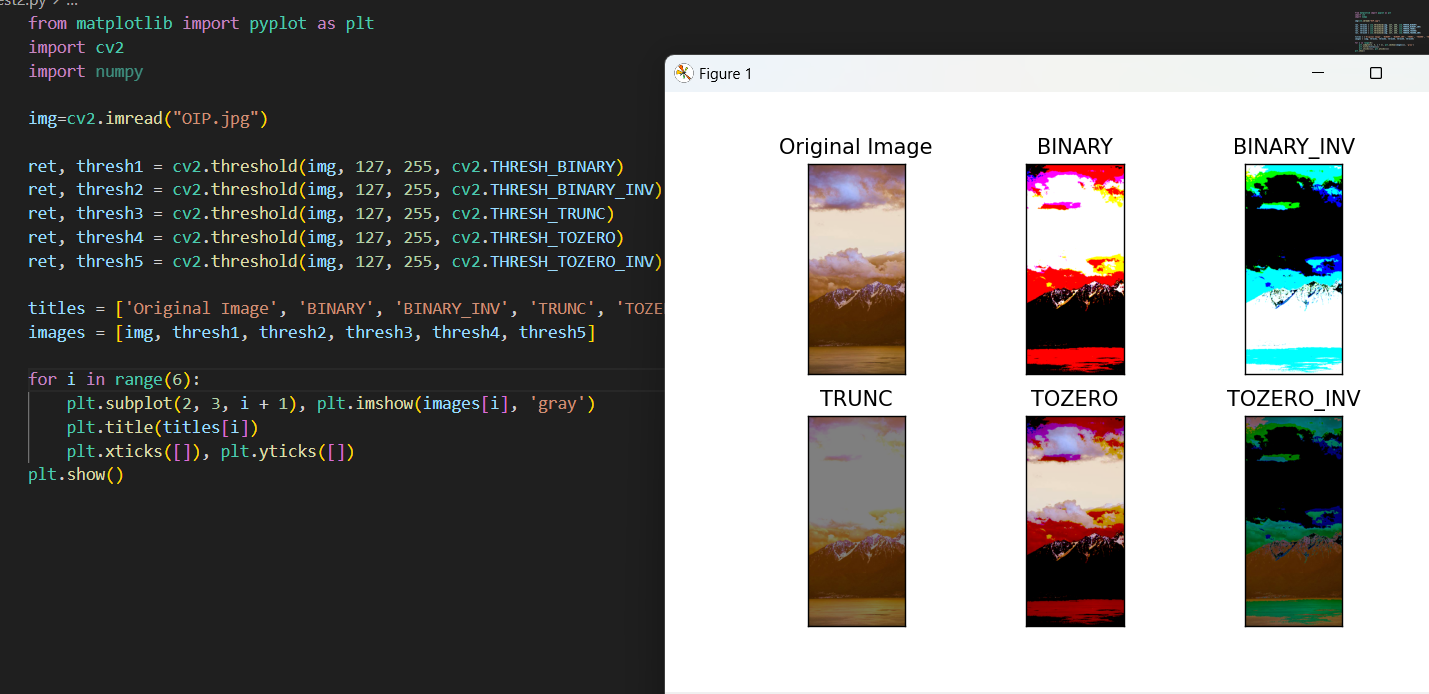
\includegraphics[width=1\textwidth]{屏幕截图 2024-09-12 194017.png}
  \caption{图片阈值}
    \end{figure}


11.图像平滑
\begin{figure}[H]
  \centering
  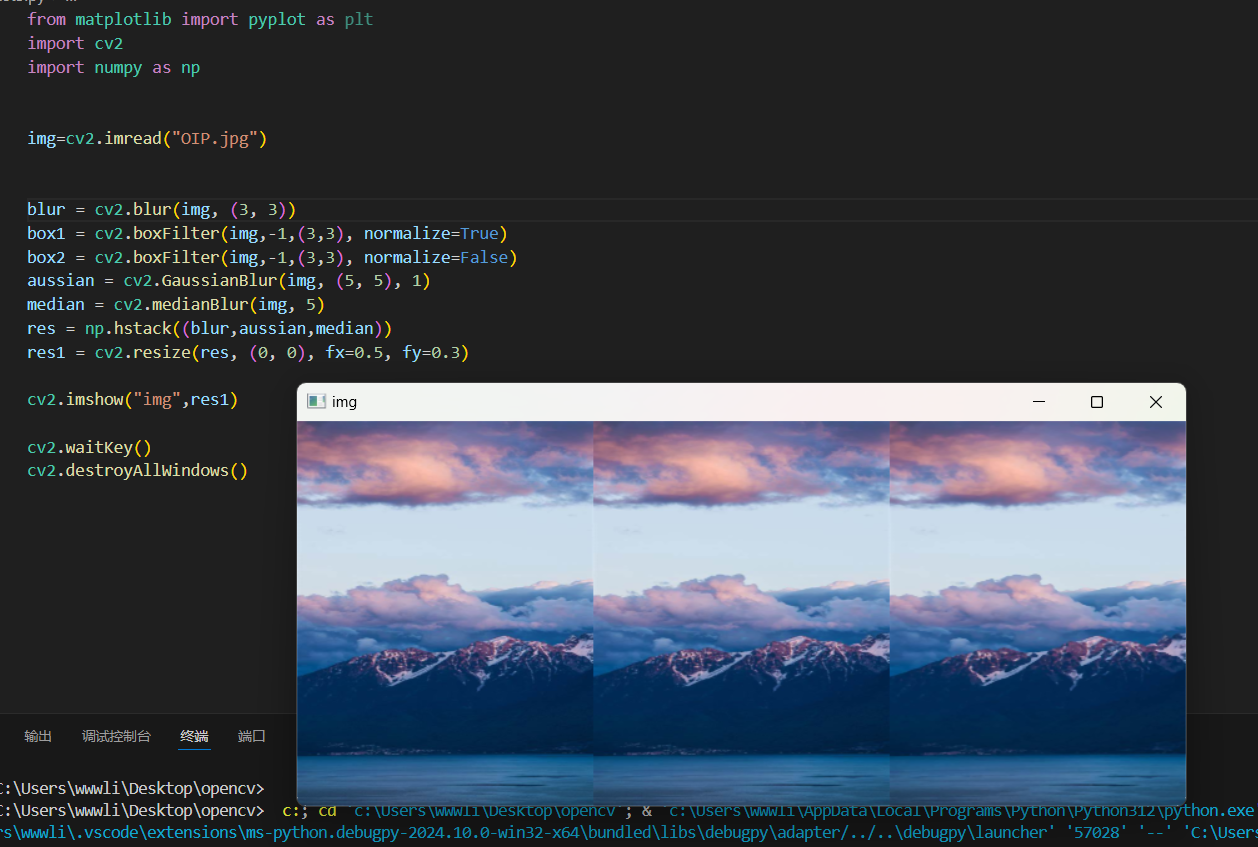
\includegraphics[width=\textwidth]{屏幕截图 2024-09-12 200700.png}
  \caption{图像平滑}
\end{figure}

12.图片的腐蚀操作
\begin{figure}[H]
  \centering
  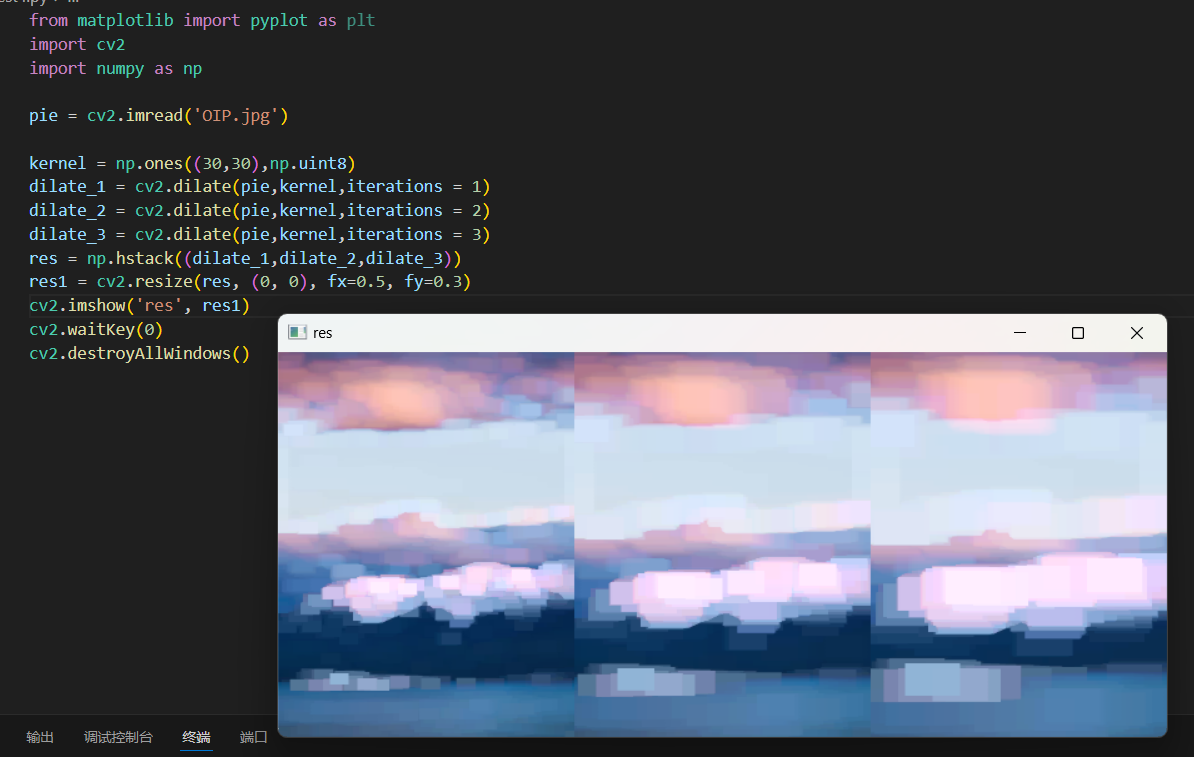
\includegraphics[width=\textwidth]{屏幕截图 2024-09-12 201525.png}
  \caption{图片的腐蚀操作}
\end{figure}

13.图片的膨胀操作
\begin{figure}[H]
  \centering
  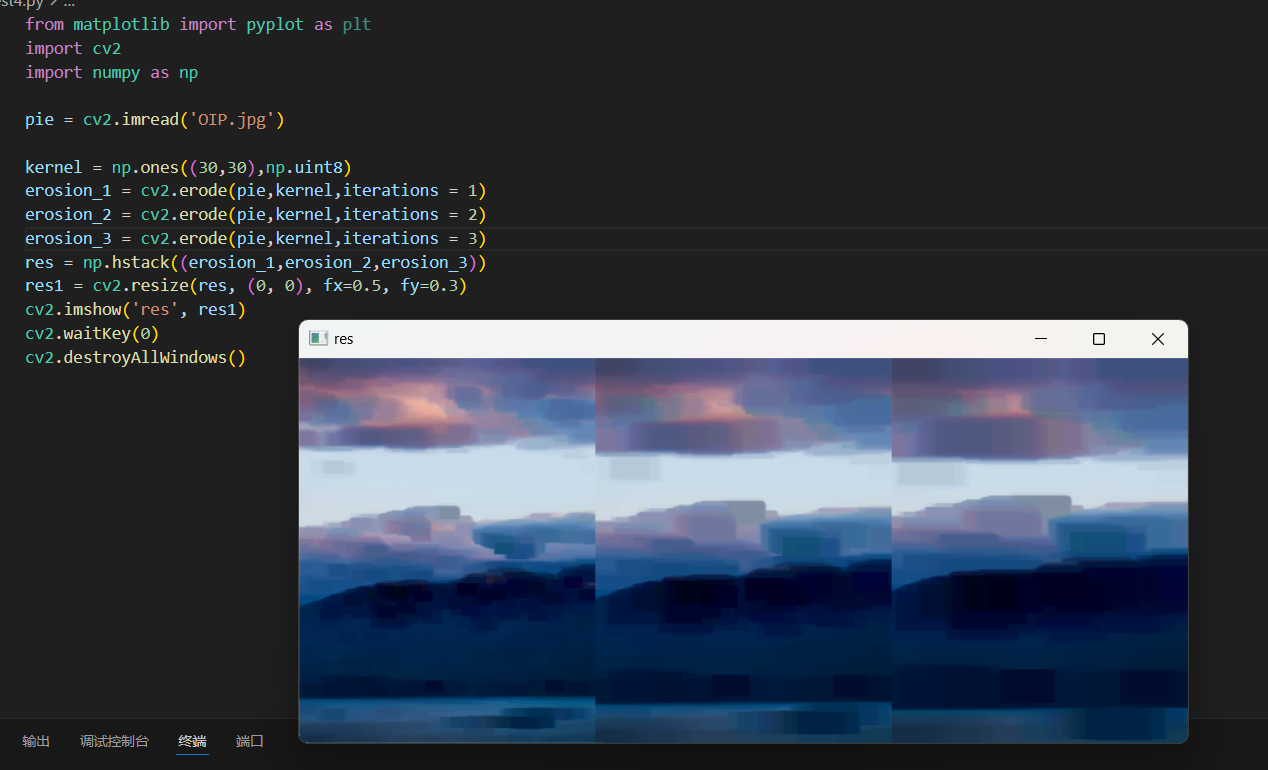
\includegraphics[width=\textwidth]{屏幕截图 2024-09-12 201917.png}
  \caption{膨胀}
\end{figure}

14.梯度运算
\begin{figure}[H]
  \centering
  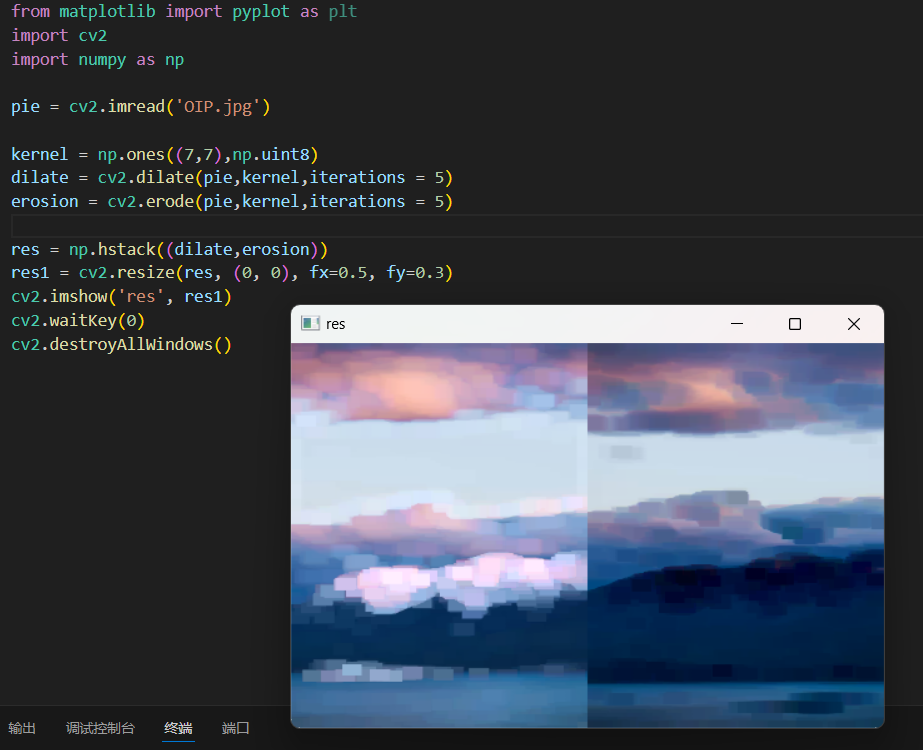
\includegraphics[width=\textwidth]{屏幕截图 2024-09-12 202112.png}
  \caption{梯度运算}
\end{figure}

\section{个人心得}

学习Python视觉应用时,我掌握图像处理的基础操作,如图像读取、显示、格式转换等。通过使用OpenCV、PIL等库,可以快速上手图像处理,并结合实践项目如人脸识别和边缘检测,加深对技术的理解。尤其是在调试过程中,多次实验调整参数是找到最佳方案的关键。同时,结合深度学习框架,如TensorFlow和PyTorch,可以进一步完成复杂的视觉任务。
\\
\indent 在命令行操作中,掌握基础的Shell命令以及如何通过Python进行自动化任务编写,是高效开发的重要途径。使用argparse或click库可以让Python脚本支持命令行参数,自定义行为,并通过虚拟环境工具(如venv或conda)管理依赖,确保项目独立性。在性能调试方面,通过命令行监控系统资源占用,可以帮助优化程序运行效率。
\\
\indent 总结来看,在学习Python视觉应用和命令行工具的过程中,动手实践是必不可少的,理论与实践相结合才能快速提升。同时,系统性学习,从基础到复杂逐步扩展知识领域,结合工具的灵活运用,会极大提高学习效率和项目开发的效果。

\section{github账户}
\href{https://github.com/newbeginnerlzh/git-task01.git}{\color{red}https://github.com/newbeginnerlzh/git-task01.git}
\end{document}
